\documentclass[12pt]{article} 
\usepackage[utf8]{inputenc}
\setcounter{secnumdepth}{4} 
\setcounter{tocdepth}{4}
\usepackage[
backend=biber,
style=alphabetic,
sorting=ynt
]{biblatex}
% add bibliography-file
\addbibresource{bibliography.bib}
% used to fix some 'overfull hbox in bibliography'
\emergencystretch=1em
% used for code listings
\usepackage{listings}
\lstset{language=Python}
\lstdefinestyle{mystyle}{
    breaklines=true,
    showspaces=false,
    showstringspaces=false,
    numbers=left,
    %numbersep=5pt,
    captionpos=t,
    %frame=shadowbox,
    basicstyle=\ttfamily\small,
}
\lstset{style=mystyle}

% to embed graphics
\usepackage{graphicx}
\graphicspath{ {./images} }
\usepackage{float} % to keep figures at the exact position in LaTex code!, see https://en.wikibooks.org/wiki/LaTeX/Floats,_Figures_and_Captions

\usepackage[all]{nowidow} %verhindert Schusterjungen und Hurensöhne 

\usepackage{times}
\usepackage[hidelinks]{hyperref}
\usepackage[onehalfspacing]{setspace}
\pagenumbering{arabic}
\usepackage{geometry}
 \geometry{
 a4paper,
 left=25mm,
 right=30mm,
 top=25mm,
 bottom=20mm,
 }
%German-specific commands
%--------------------------------------
\usepackage[ngerman]{babel}
\usepackage{csquotes}
%--------------------------------------
%Hyphenation rules
%--------------------------------------
\usepackage{hyphenat}
\hyphenation{Mathe-matik wieder-gewinnen}
%--------------------------------------
%Inhaltverzeichnis Benennung
%--------------------------------------
\renewcommand{\contentsname}{Inhaltsverzeichnis}
%--------------------------------------

\title{KOL Floyd Erdmann}
\author{Floyd Erdmann}
\date{October 2021}

\begin{document}
\pagenumbering{gobble}
\setlength{\baselineskip}{5mm}
\maketitle
\onehalfspacing

\newpage
\tableofcontents
\newpage
\listoffigures
\lstlistoflistings
\newpage
\pagenumbering{arabic}
\setcounter{page}{5}
\section{Einleitung}
Der Coronavirus beeinflusst, verändert und zerstört weltweit seit über zwei Jahren das Leben von Milliarden von Menschen. Eine ähnlich verheerende Pandemie forderte vor 104 Jahren, mit Ende des ersten Weltkrieges, bis zu 50 Millionen Leben. In dieser Arbeit wird der Autor Analogien, Unterschiede und deren Ursachen der Pandemien darlegen und begründen. Im Vordergrund steht dabei die Auswirkung der Globalisierung auf den Verlauf und die Gegenmaßnahmen der aktuellen Covid-19-Pandemies im Vergleich zur Spanischen Grippe. Um Ursachen und Wirkungen fundiert aufzeigen und begründen zu können, wird der Verfasser zunächst auf Grundlagen der Krankheitsübertragung und Globalisierung eingehen um im Anschluss Spanische Grippe und Covid-19 hinsichtlich ihrer Krankheitsverläufe, Ausbreitung und Gegenmaßnahmen zu vergleichen und entscheidende Faktoren herrauszustellen, welche für Differenzen in genannten Kriterien geführt haben. Im Eigenanteil dieser Arbeit veranschaulicht der Autor die Auswirkung von krankheitsspezifischen Faktoren und Abstandsregelungen anhand einer programmierten Simulation basierend auf dem SEIR-Modell. Diese wird im Anschluss anhand unterschiedlicher Szenarien ausgewertet und erklärt um dem Leser die Vorgehensweise des Autors näherzubringen. Als Motivation zur Erstellung dieser Arbeit bezieht der Autor aus der derzeitige Relevanz des Themas, der starken Auswirkung auf den Alltag aller Menschen sowie aus der medialen und politischen Brisanz. Weiterhin war dem Verfasser unklar wie Covid-19 trotz fortgeschrittener Technologie und Medizin ähnliche Infektionszahlen aber durtlich geringere Todesopfer als die Spanische Grippe aufweist.

\newpage
\section{Krankheitserreger}\label{sec:Krankheitserreger}
\subsection{Überblick der wichtigsten Krankheitserreger beim Menschen}
Der Überbegriff „Krankheitserreger“, in der Medizin auch „Keime“ oder „Infektionserreger“, steht für subzelluläre Erreger oder Mikroorganismen, welche in anderen Organismen gesundheitsschädigende Abläufe verursachen. Beim Menschen wird grundsätzlich zwischen den vier am meisten verbreiteten Erregerarten unterschieden:
\begin{itemize}
    \item \subsubsection{Bakterien}
    Bakterien bilden die einfachste Lebensform auf dem Planeten Erde. Sie sind einzellige Kleinstlebewesen und werden den Prokaryoten, den Lebewesen ohne Zellkern zugeordnet.\footnote{Vgl. \cite{Nagel2021}} Mit einem Durchmesser von 0,1 bis 700 Mikrometer\footnote{Vgl. \cite{BZgA2021}} sind sie um ein Vielfaches größer als Viren. Infektionskrankheiten, welche durch Bakterien ausgelöst werden, sind u. a. Keuchhusten und Blutvergiftung, Salmonel- oder Tuberkulose.
    \item \subsubsection{Viren}
    Da Viren im Gegensatz zu Bakterien weder aus einer eigenen Zelle bestehen noch einen eigenen Stoffwechsel betreiben, werden sie von Virologen nicht zu den Lebewesen zugeordnet, sondern als organische Struktur bezeichnet. Aufgrund ihrer Fähigkeit zur Evolution werden sie jedoch trotzdem als „dem Leben nahestehend“ betrachtet. Viren bestehen nur aus ihrem Erbgut, der DNA oder RNA, sowie aus Proteinen und brauchen daher eine Wirtszelle um sich zu vermehren.
    \item \subsubsection{Parasiten}
    Als Parasiten bezeichnet man Lebewesen, welche auf oder in einem Organismus einer anderen Art, dem Wirt, leben und/oder Nahrung von diesem beziehen. Der Wirt bleibt dabei in der Regel am Leben, wird jedoch in seiner Gesundheit oder seinem Wohlbefinden geschädigt. Krankheiten, welche durch Parasiten am Wirt hervorgerufen werden, bezeichnet man als Parasitosen. 
    \item \subsubsection{Pilze}
    Pilze sind eigenständige Lebewesen mit einem sehr vielseitigen Erscheinungsbild. Sie können sowohl in der Umwelt als auch in einem Wirt existieren und leben auf der menschlichen Haut, indem sie sich von abgestorbenen Zellen ernähren. Krankheiten, welche unter bestimmten Bedingungen wie Schwächung des Immunsystems durch Pilze hervorgerufen werden, bezeichnet man medizinisch als Mykosen.
    
\end{itemize}
Eine Ansteckung mit einem der genannten Krankheitserreger nennt man Infektion. Hierbei bilden die Parasiten eine Ausnahme, da der Befall eines Organismus mit einem Parasiten als Infestation bezeichnet wird.

\subsection{Übertragungswege der Krankheitserreger}
Die Art und Weise und Wahrscheinlichkeit einer Übertragung von Krankheitserregern ist durch die Diversität der Eigenschaften dieser stark beeinflusst. Außerdem führt nicht jede Übertragung eines Keims auch zu einem symptomatischen Krankheitsverlauf, da das Imunsystem Erreger teils ohne auftretende Nebenwirkungen abtöten kann. Beim Menschen wird grundsätzlich in folgende Übertragungswege unterschieden:
\begin{itemize}
    \item \subsubsection{Tröpfcheninfektion}
    Bei der Infektion durch Sekret-Tröpfchen wird Atemwegssekret durch Niesen, Husten oder Sprechen in die Umgebung freigesetzt. Diese Tröpfchen können Krankheitserreger enthalten und eine gesunde Person anstecken, falls diese durch die Schleimhäute im  Mund, der Nase oder der Augen in den Körper aufgenommen werden. Durch diesen Übertragungsweg werden vorallem Atemwegserkrankungen wie Keuchhusten weitergegeben. Auch Infektionen der Grippe und des Covid-19 Virus erfolgen meist über eine Tröpfcheninfektion. Vorbeugende Maßnahmen dafür sind das Minimieren von Kontakten, gute Hygiene und gegebenenfalls das Tragen einer Mund-Nasen-Bedeckung.
    Fälschlicherweise wird die „Übertragung durch die Luft“ häufig als eigenständiger Übertragungsweg erwähnt, dabei handelt es sich ebenfalls um eine Tröpfcheninfektion durch sehr kleine, teilweise stundenlang in der Luft schwebende Sekret-Tropfen. Wie schnell Tröpfchen und Aerosole in der Luft schweben oder absinken ist dabei stark von der Luftbewegung, der Luftfeuchtigkeit und der Belüftung abhängig.\footnote{Vgl. \cite{Rki21}}
    \item \subsubsection{Schmierinfektion}
    Eine andere Weitergabemöglichkeit von Krankheitserregern ist die Kontaktübertragung mittels Berührung. Dies kann sowohl von Mensch zu Mensch als auch über den Kontakt mit verunreinigten Gegenständen erfolgen. Der Aufbau des Erregers und die Beschaffenheit der Oberfläche spielen hierbei eine große Rolle, da sie entscheidend für die Lebensdauer von Viren und Bakterien auf Objekten sind.
    \item \subsubsection{Übertragung durch Lebewesen}
    Infektionskrankheiten wie Borreliose können von einem infizierten Tier, welches als Träger des Krankheitserregers dient, auf einen Menschen übertragen werden. Das Tier muss bei diesem Übertragungsweg nicht zwangsweise erkrankt sein. Häufig auftretende Beispiele sind Borreliose durch Zeckenstiche, Tollwut und Ebola.
    \item \subsubsection{Übertragung durch Lebensmittel}
    Wenn Lebensmittel, welche von Krankheitserregern befallen sind, von Menschen verzehrt werden, kann dies eine Erkrankung auslösen. Häufig handelt es sich dabei um eine Diarrhoe. In Deutschland sind vor allem Bakterien wie Salmonellen und Listerien sowie Noro- und Rotaviren für eine Infektion durch Lebensmittel verantwortlich.
    \item \subsubsection{Übertragung durch Wasser}
    Krankheitserreger können über das Wasser durch verschiede Wege in den menschlichen Körper gelangen. Eine Infektion über das Trinkwassser kann auch der Übertragung durch Lebensmittel zugeordnet werden, allerdings ist eine Übertragung von Krankheiten wie Campylobacter und EHEC auch durch das Baden in verunreinigten Gewässern möglich und stellt somit eine eigene Übertragungsvariante dar.
\end{itemize}
Eine Übertragung von Krankheitserregern kann also durch körperliche Nähe und den daraus erfolgenden Austausch von Erregern über Körperflüssigkeiten, verunreinigte Gegenstände, Lebensmittel oder Wasser sowie über andere Lebewesen erfolgen.
\subsection{Vermehrung von Krankheitserregern}
Im Kontext dieser Komplexarbeit befasst sich der Autor ausschließlich mit der Verbreitung von Viren, da das Hauptaugenmerk dieser Ausarbeitung auf dem Zusammenhang von Viren mit der Globalisierung gelegt wird.

\subsubsection{Vermehrung von Viren}
Um sich zu vermehren, benötigen Viren eine Wirtszelle eines lebenden Organismus, da der Virus selbst zu keinem Stoffwechselvorgang fähig ist. Die Vermehrung kann in zwei Arten unterschieden werden. Beim lytischen Zyklus, welcher stets den Tod der befallenen Zelle als Folge hat, schleust das Virus seine Nukleinsäure in die Wirtszelle ein, während beim lysogenischen Zyklus die Replikation des Virus meist ohne den Zelltod stattfindet. Bei dieser Art der Vermehrung wird die genetische Information des Virus in das Wirtsgenom integriert, was die Entstehung eines Provirus zur Folge hat. Um den Vermehrungsprozess zu beginnen, heften sich Viren bei beiden Übertragungsarten an die Zellmembran um in der anschließenden Phase der Penetration das Viruserbgut in die Zelle freizusetzen. Dies ist über die Fusionierung, dem Verschmelzen der Virushülle mit der Zellmembran der Wirtszelle und anschließenden Abgabe des Erbgutes ins Zellinnere, oder den der Endozytose, dem Absenken des Virus in die Zellmembran der Wirtszelle durch welches ein Vesikel entsteht, das den Virus ins Zellinnere transportiert, möglich. Zellmaschinerien, welche normalerweise das Erbgut der Wirtszelle ablesen, haben nun auch Zugriff auf das Viruserbgut, womit eine wichtige Voraussetzung für die Virusvermehrung gegeben ist. In der darauffolgenden Phase produziert die Wirtszelle anhand des eingeschleusten Erbguts neue Virusproteine und Viruserbgut und stellt somit alle einzelnen Bestandteile eines Virus in großer Zahl her. Eine Polio-infizierte Zelle stellt circa 1000 neue Viren pro Zelle her. Die Einzelteile des neu produzierten Virus sind in der Lage sich von selbst zu einem kompletten Virus zusammenzusetzen. Den Abschluss einer erfolgreichen Virusvermehrung stellt die Freisetzung dieser dar. Durch das Schädigen der Zelle mit dessen Tod als Folge und dadurch erfolgende Freisetzung des Virus, der Knospung, bei welcher der Virus mit Abschnitten der Zellmembran abgeschnürt wird oder der Sekretion, dem Abschnüren in das Innere der Organellen und anschließende Freisetzung des Virus durch Vesikel, wird die Vermehrung des Virus vollendet.

\section{Globalisierung der letzten 100 Jahre}\label{sec:Globalisierung}
\subsection{Globalisierung als Prozess}
Globalisierung bezeichnet einen Prozess, in dem weltweite Verflechtungen in vielen Bereichen, wie Wirtschaft, Politik, Kultur, Umwelt und Kommunikation, zwischen Individuen, Gesellschaften, Institutionen und Staaten zunehmen. Als wesentliche Gründe gelten der technische Fortschritt mit wichtigen Innovationen in Produkt- und Prozessbereichen, sowie in Kommunikations- und Transporttechnologien, die ordnungspolitische Grundorientierung mit Entscheidungen und Maßnahmen zur Liberalisierung des Welthandels und das Bevölkerungswachstum in 229 von 235 Staaten seit 1950. Kennzeichnend für Globalisierung ist die Zunahme an Verbindungen zwischen Gesellschaften und Problembereichen. Dies geschieht unter numerischer Zunahme, qualitativer Intensivierung und einer räumlichen Ausdehnung. Es kann in folgende Arten der Globalisierung unterschieden werden:
\begin{itemize}
    \item \subsubsection{Ökonomische Globalisierung}
    Mit einer Steigerung des weltweit statistisch erfassten Warenexportes um mehr als das 19-fache im Zeitraum von 1960 bis 2017 ist die Globalisierung in starkem Maße ökonomischer Natur. Trotz enormem Zuwachs des weltumspannenden Handels und Expansion der transnationalen Unternehmen durch große Kapitalströme, ermöglicht durch Abbau von Regulierungen im Wirtschafts- und Finanzbereich, kann man die Wirtschaft noch nicht als vollständig global bezeichnen, da lediglich 20\% der Güter und Dienstleistungen international gehandelt werden. Zusätzlich sind derzeit nur circa 30\% der Weltbevölkerung in die Weltwirtschaft integriert. Der Begriff „Welthandel“ ist auch deshalb irreführend, da der Einfluss ganzer Kontinente, beispielsweise Afrika und Südamerika, sich auf einen einstelligen Prozentsatz beläuft. Entwicklungsländer in diesen Kontinenten sind aufgrund von politischer Instabilität, mangelhafter Rechtssicherheit und unzureichender Infrastruktur meist vom Globalisierungsprozess ausgeschlossen. Weitherhin ist die Globalisierung anhand der verstärkten Abkopplung der Finanzmärkte von der realwirtschaftlichen Entwicklung zu erkennen, wodurch es zu gehäuften kurzfristigen Kapitalanlagen der spekulativen Art kommt und Finanzmärkte zum „Handlungsort der neuen Gestaltung der Welt werden“ \footnote{Vgl. \cite{Renz2001}}. Zur Globalisierung der Wirtschaft zählt außerdem die Veränderung in Transport- und Personenverkehr. Trotz steigender Anzahl der Containerschiffe im Weltseehandel wuchs auch die Kapazität derer in den letzten 40 Jahren um 2500\%\footnote{Vgl. \cite{Keller2021}}. Diese Entwicklung des Transportwesens wirkt sich nicht nur positiv, durch eine Zunahme von Arbeitsplätzen, aus sondern bringt auch schwerwiegende Probleme, zum Beispiel ökologischer Natur, mit sich. Mit Ausweitung der Zug-, Automobil- und Luftverkehrsnetze weiten sich Personenverkehr und Tourismus grenzüberschreitend aus. Ein letzter wichtiger Aspekt der ökonomischen Globalisierung, welcher in den letzten Jahrzehnten ein enormes Ausmaß angenommen hat, ist die Kommunikation und das Internet. Mit einer seit 1960 Verzehnfachung der Telefonanschlüsse im weltweiten Telefonnetz und einem Anstieg der Internetnutzer um fast 50\% in den letzten 15 Jahren\footnote{Vgl. \cite{Rabe2021}} ist es einfacher global zu kommunizieren als je zuvor.
    \item \subsubsection{Politische Globalisierung}
    % overfull hbox, Lösung siehe Antwort 2: https://tex.stackexchange.com/questions/111948/what-is-a-overfull-hbox-9-89561pt-too-wide
    \begin{sloppypar}
    Die Globalisierung der Politik resultiert aus den Folgen der wirtschaftlichen und kulturellen Gloablisierung. Durch Hürden in den Problemfeldern Wirtschafts-, Natur- und Sicherheitspolitik ist eine globale Kooperation in vielen Fällen unumgänglich, da die begrenzten nationalen Möglichkeiten zur Problembewältigung nicht ausreichen. Zwei mögliche Lösungswege werden diskutiert um diesen Schwierigkeiten entgegenzuwirken. Der Versuch Globalisierung zu verhindern und zu einem gewissen Grad zurückzudrehen um durch Regionalismus eine Gegenmacht zu bilden und den an den Markt verlorenen Einfluss zurückzugewinnen, stellt den ersten Lösungsweg dar. Ein anderer Ansatz ist der Versuch, globalpolitische Strukturen und Regelwerke zu kreieren um künftige Herausforderungen zu bewältigen. Drei Ebenen auf welche sich die politische Globalisierung bezieht, sind die Zunahme von internationalen Verträgen, Vereinbarungen und ein Anstieg der internationalen Öffentlichkeit mit einer auf globale Ereignisse ausgerichtete Berichterstattung. Die Globalisierung der Politik sorgt einerseits für internationale Zusammenarbeit und Organisationen wie UNO, WELTBANK und IWF kreiert aber andererseits einen steigenden Konkurrenzkampf zwischen den einzelnen Nationalstaaten.
    \end{sloppypar}
    \item \subsubsection{Gesellschaftliche und Kulturelle Globalisierung}
    \begin{sloppypar}
    Auch die gesellschaftliche und kulturelle Globalisierung hängt stark von der wirtschaftlichen Globalisierung ab. Die Diffusion unterschiedlicher Kulturen, welche während der Zeit des Kolonialismus durch Inbesitznahme fremder Territorien und Unterwerfung der ansässigen Bevölkerung stattgefunden hat und heutzutage vor allem durch Tourismus und moderne Massenkommunikationsmittel fortgeführt wird, steht dabei im Vordergrund. Um trotz wirtschaftlicher Globalisierung größtmöglichen Profit zu erzielen, versuchen transnationale Unternehmen Teil der jeweilig vorherrschenden Kultur zu werden. Die Auswirkungen der Globalisierung der Kultur äußern sich durch eine stetig steigende Anzahl bikultureller Partnerschaften und nach UN-Schätzungen circa 281 Millionen Migranten weltweit.\footnote{Vgl. \cite{WMR2020}} Eine weitere Folge ist in der Globalisierung der Sprache zu erkennen. So breitet sich der Gebrauch der englischen Sprache stetig aus\footnote{Vgl.\cite{Sprache2016}} und Exonyme verschwinden zunehmend aus Nationalsprachen.
    \end{sloppypar}
    \item \subsubsection{Ökologische Globalisierung}
    Einhergehend mit positiven Auswirkungen der Globalisierung, wie einem weltweit steigenden Pro-Kopf Einkommen\footnote{Vgl. \cite{Lammar2013}}, stetig steigenden Lebenserwartungen\footnote{Vgl. \cite{Radtke2021}} und besser ausgebauter Infrastruktur, verschärfen sich jedoch auch die ökologischen Probleme. Zwar steigt aufgrund der Globalisierung die Wahrnehmung für global auftretende Schäden und Industrieländer schaffen Umweltstandards und strenge Umweltgesetze\footnote{Vgl. \cite{WikipGlobWirtsch}}, diese können allerdings von Schwellen- und Entwicklungsländern nicht eingehalten werden. Aufgrund des Wettbewerbdrucks der wirtschaftlichen Globalisierung erlangen vordergründig Staaten Vorteile, welche Umweltstandards und Auflagen niedrig ansetzen oder sogar bestehende Regulierungen aufheben. Der Welthandel und der damit verbundene Transportaufwand und die Warenherstellung hat außerdem zu einem enormen Energieverbrauch geführt. Laut einer Studie von „Our World in Data“ belief sich der Anteil von Energiegewinnung an der Gesamtheit der globalen Treibhausgasemissionen auf über 70 Prozent\footnote{Vgl. \cite{Ritchie2021}}. Da sich Nationalstaaten bei Zusammentreffen wie den Klimagipfeln sehr schwer tun notwendige Schritte einzuleiten und Abkommen zu vereinbaren um zukünftige Umweltkatastrophen abzuwenden, bildeten sich in den letzten Jahrzehnten diverse Nichtregierungsorganisationen (NGO) wie Greenpeace und Amnestie International, welche mithilfe ihres Einflusses Druck auf Regierungen ausüben um verschiedene Ziele zu forcieren\footnote{Vgl. \cite{Ehrlich1966} }.
\end{itemize}
\subsection{Chancen und Risiken der Globalisierung}
\subsubsection{Chancen}
Eine der wichtigsten Chancen der Globalisierung ist die Durchsetzung der Menschenrechte in einem internationalen Rahmen. Zwar gibt es bis heute Staaten, in welchen es immer noch zu schwerwiegenden und teils systematischen Menschenrechtsverstößen kommt, jedoch hat sich der globale Zustand dank Einfluss der Industrie- auf Entwicklungsländer und modernen Kommunikationsmitteln deutlich verbessert.\footnote{Vgl. \cite{Lohrmann} und \cite{WikipMenschRechte}} 
Eine weitere Gelegenheit für Fortschritt durch Globalisierung lässt sich im potenziellen Weltfrieden erkennen. Auf Basis der Staatsform Demokratie in vielen entwickelten Ländern und internationalen Bündnissen und Verträgen entsteht ein friedliches Verhältnis zwischen Nationen. Um dies zu erreichen muss die Außenpolitik demokratisch gesinnter Staaten jedoch mithelfen, Demokratie in anderen Ländern zu erreichen. Dass dieses Ziel noch lange nicht erreicht ist, kann man an politischen Spannungen wie beispielsweise zwischen China und Taiwan erkennen.
Aus ökonomischer Sicht stellt die Globalisierung eine große Chance dar, da durch einen Anstieg im Handel und verstärkte Arbeitsteilung Armut durch Arbeitsplätze bekämpft werden kann. Dies lässt sich durch den Anstieg der weltweiten Exporte im Warenhandel seit 1950\footnote{Vgl. \cite{Urmersbach2021}} und steigendem Wohlstand mit höheren Lebenserwartungen erkennen. Diese Entwicklung beinhaltet auch den Rückgang der Anzahl von in absoluter Armut lebender Menschen\footnote{Vgl. \cite{Roser2016}}.
Eine positive Entwicklung stellt die vermehrte Toleranz und der Austausch unterschiedlicher Kulturen dar. Trotz der erwähnten Diffusion, bleiben mit den jeweiligen Kulturen einhergehende Praktiken und Formen des Ausdrucks erhalten und werden sogar in andere Kulturen übernommen. So müssen Filmproduktionsgesellschaften drauf achten, Filme für ein heterogenes Publikum zu produzieren und Diskriminierung in keiner Weise zu unterstützen um größtmögliches Profitpotential zu erreichen. Somit führt Globalisierung indirekt zu einer zunehmend toleranteren Welt. Eine weitere Form des Umdenkens lässt sich im Zusammenhang mit der ökologischen Globalisierung erkennen, da durch moderne Kommunikationsmittel ein „planetares Bewusstsein“\footnote{Vgl. \cite{WikipGlobWirtsch}} begünstigt wird.
\subsubsection{Risiken}
Globalisierungsskeptiker kritisieren die globale Integration heftig und sehen eine große Bedrohung in der vom Markt beherrschten Welt.\footnote{Vgl. \cite{Renz2001}} Ein schwerwiegender Kritikpunkt ist, dass die Globalisierung für eine Vernachlässigung von Menschen- und Arbeitnehmerrechten, ökologischen Standards und Demokratie verantwortlich sei und nur Märkte und Geschäftsbeziehungen fördere.\footnote{Vgl. \cite{IntGB2010}} Das Individuum habe demnach, durch die  Macht des Marktes, keinen Einfluss mehr. Dies sorgt vor allem bei ökologische denkenden Aktivisten für großen Unmut.
Ein großes Risiko für die bisherige Grundidee des Wohlfahrstaates ist der ansteigende Modernisierungsdruck. Der Steuersenkungswettlauf um in der modernen Wirtschaft mithalten zu können, sorgt für minimale Staatseinnahmen, wodurch wohlfahrtstaatliche Leistungen unbezahlbar werden. Die stetige Zunahme der Lebenserwartung und damit einhergehend längere Rentenzahlungen sowie Behandlungs- und Medikamentkosten benötigten eine Entwicklung in die entgegengesetzte Richtung.\newline

Die zurzeit wohl populärste negative Auswirkung und eins der größten Risiken für die Zukunft der Menschheit sind die Umweltschäden infolge der Globalisierung. Besorgnis erregend ist dabei das Tempo der Verhandlungsfortschritte bei internationalen Klimakonferenzen. So gab es bereits 1979 eine erste Weltklimakonferenz\footnote{Vgl. \cite{Weltklimakonferenzen}}, doch erst im Jahr 2015 bei der in Paris stattgefundenen Klimakonferenz kam es zum Vertragsabschluss. Die Klimaerwärmung als Folge der Globalisierung spielt in dieser Arbeit eine besondere Rolle, da vor allem die Ausbreitung von vektorgebundenen Krankheiten wie Malaria und Leishmaniasis direkt und indirekt vom Klima beeinflusst ist.\footnote{Vgl. \cite{Ebert2005}}

\section{Spanische Grippe und Coronavirus}\label{sec:GrippeUndCovid}
Vor 104 Jahren verbreitete sich eine Influenza-Pandemie, welche mit 50 Millionen Todesfällen zur verheerendste Pandemie der Geschichte wurde. %Inwiefern sich Verlauf und die Verbreitung des Subtypes A/H1N1, der "spanischen Grippe", dem aktuellen Covid-19-Virus ähnelt wird der Autor in diesem Vergleich offenlegen.
Trotz einer Weltbevölkerung von nur 1,8 Milliarden Menschen und einer nicht annähernd so fortgeschrittenen Globalisierung wie 2021 forderte die Spanische Grippe somit deutlich mehr Todesopfer als das derzeit kursierende Coronavirus.
\subsection{Zur Spanischen Grippe}
Als virueller Abkömmling des Influenzevirus, Subtyp A/H1N1, infizierte das Virus zwischen 1918 und 1920 in drei Wellen etwa 500 Millionen Menschen weltweit.\footnote{Vgl. \cite{Span}} Mit einer Letalität, der Tödlichkeit einer Erkrankung, von circa 5 bis 10\%, war die Sterblichkeit infizierter Menschen deutlich höher als bei Erkrankungen durch andere Influenza-Erreger. Zusätzlich zur hoher Sterblichkeitsrate wies der Erreger andere Besonderheiten wie ein großes Ansteckungsrisiko und, im Gegenstz vorherigen Influenzaviren durch welche vorallem Kleinkinder und ältere Menschen gefährdet sind, eine erhöhte Sterblichkeitsrate bei 20- bis 40-jährigen Menschen. 

\subsubsection{Krankheitsverlauf und Symptome}
Trotz von anderen Influenzaviren abweichenden Merkmalen ähnelten die spezifischen Symptome der Spanische Grippe sehr jener anderen Influenza-Erkrankungen. So begann der Krankheitsverlauf sehr plötzlich durch ein ausgeprägtes Krankheitsgefühl im ganzen Körper mit Kopfschmerzen, Glieder-, Kreuz- und Rückenschmerzen, aber auch Müdigkeit, Abgeschlagenheit und Antriebsschwäche.\footnote{Vgl. \cite{Span}} Während es bei Infektionen der ersten Welle vorallem zu milden Krankheitsverläufen mit genannten Symptomen kam, wirkte sich die zweite Welle häufig deutlich schneller und gravierender aus. Infizierte starben nur wenige Stunden nach Erstsymptomen\footnote{Vgl. \cite{Hanan2021}}, aber auch Überlebende hatten oft noch Wochen Probleme mit starker Müdigkeit und chronischer Erschöpfung. Auch die Anzahl der Infizierten mit Lungenentzündungen, hämorrhagischem Fieber und Zyanose, bläulich-schwarze Verfärbung der Haut durch Mangel an Sauerstoff, stieg mit der zweiten Welle des Virus stark. 
\subsubsection{Ausbreitung und Verlauf}
Die Spanische Grippe verbreitete sich, wie auch Influenza im Allgemeinen, durch die Weitergabe per Tröpfcheninfektion und mit einer Verringerung der Infektiösität ab 22 Grad Celcius entspricht auch die Umweltstabilität des Virus dem der Allgemeinen Influenzaerkrankung. Die Basisreproduktionszahl des Virus lag zwischen zwei und drei. Die erste, im Frühjahr 1918 in Nordamerika beginnenden, Ausbreitungswelle wies mit einer Letalität von 5 Toden pro 1000 Menschen\footnote{Vgl. \cite{Jeff06}} keine außergewöhnlich hohe Tödlichkeit auf, verbreitete sich jedoch ungewöhnlich schnell. Diese große Ausbreitungsgeschwindigkeit der ersten Welle ist unter anderem auf auf die Truppenbewegungen, vorallem dem Überqueren des Atlantiks durch Streitkräfte der Vereinigten Staaten, der Soldaten im ersten Weltkrieg, welcher 1918 sieben Monate nach der Entdeckung der spanischen Grippe endete, zurückzuführen. 
Die Ende August beginnende zweite Welle stellte nicht nur Krankenhäuser und Ärzte, sondern auch die Wirtschaft vor eine riesige Herausforderung. Während die erste Welle nur circa drei bis fünf Millionen Menschen tötete sorgte die zweite Welle mit bis zu 50 Millionen Todesopfern für globales Chaos. In Europa lag der Fokus der Presse jedoch nach wie vor auf dem ersten Weltkrieg lag und die Versorgungslage befand in vielen Staaten in einem sehr schlechten Zustand. In Indien, stark beeinflusst durch eine Hungersnot,  wird die Letalitätsrate während der zweiten Welle auf bis zu fünf Tote je einhundert Einwohnern und die Anzahl der Toten auf bis zu 20 Millionen geschätzt.\footnote{Vgl. \cite{Bax20}} Gründe für die hohe Verbreitungsgeschwindigkeit der zweiten Welle waren weiterhin reisende Soldaten, die Vermeidung von Quarantänisierung infizierter Personen während des Krieges und aufgrund überfüllter Krankenhäuser und dem Fehlen eines wirksamen Gegenmittels.
Ab Februar 1919 gab es in vielen Staaten erneut eine, weitaus harmlosere, Grippewelle, welche aufgrund der sehr jungen Todesopfer ebenfalls der Spanischen Grippe zugerechnet wird. Da der Virus ab dem Jahre 1920 deutlich weniger tödlich und Grippewellen der folgenden Jahre von weitaus geringerem Ausmaß und anderer Altersverteilung geprägt waren gelten diese Jahre als das Ende der Pandemie.
\subsubsection{Reaktionen und Gegenmaßnahmen}
Bereits mit Ende der ersten Welle leiteten erste Länder Quarantänemaßnahmen ein, Zeitungen warnten vor Symptomen und Doktoren rieten zu Abstand und Hygiene. Jedoch waren Quarantäneanordnungen von Schiffen aufgrund des Krieges nicht umsetzbar, Verschwörungstheorien und der Fakt, dass keine wirkende Impfung gegen die spanische Grippe existierte erschwerten den Prozess des Aufhaltens der Pandemie.\footnote{Vgl. \cite{Hist10}} Global verbreiteten sich Empfehlungen um eine Infektion zu vermeiden. So empfahl die Zeitung "Douglas Island News" im November 1918 Menschenmengen zu meiden, häufig zu lüften, eine Maske zu tragen, sich warm zu halten und den Mund nicht zu berühren.\footnote{Vgl. \cite{Mai2021}} Obwohl spätere Studien zeigten, dass die Mund-Nasen-Schutzpflicht und das Verbot von Massenveranstaltungen die Todesrate in diversen amerikanischen Großstädten um bis zu 50\% senkte stießen diese Einschränkungen nicht in allen Teilen der Bevölkerung auf Zustimmung.

\subsection{Zur COVID-19-Pandemie}
Die erstmals im Dezember 2019 in Wuhan beschriebene Infektionskrankheit, welche durch den Virus SARS-CoV-2 hervorgerufen wird, infizierte innerhalb von zwei Jahren mehr als 300 Millionen Menschen mit Fällen in jedem derzeit existierenden Staat. Trotz einer deutlich geringeren Tödlichkeit als die Spanische Grippe erlagen bereits 5,5 Millionen Menschen der Krankheit weltweit. 
\subsubsection{Krankheitsverlauf und Symptome} \label{subsec:Cov-Verlauf}
 Nach einer durchschnittlichen Inkubationszeit von circa fünf bis sechs Tagen treten meist Symptome wie Husten, Schnupfen, Fieber, Gliederschmerzen, Geruchs- und Geschmacksverlust und Abgeschlagenheit auf. Sowohl in der Art der Hauptsymptome als auch in der großen Anzahl der weniger häufigen Krankheitserscheinungen gleichen sich Covid 19 und die Spanische Grippe sehr.\footnote{Vgl. \cite{Gov21}} Die genannten Symptome klingen in circa 81\% der Fälle innerhalb von zwei Wochen ohne größere Komplikationen wieder ab, bei schwereren Verläufen entwickelt sich jedoch in der zweiten Krankheitswoche aufgrund einer Infektion der unteren Atemwege bis zur Lungenentzündung eine schwere Atemnot. In diesem Fall kann aufgrund von Versagen der Atem- und Kreislauffunktion eine intensivmedizinische künstliche Beatmung und externe Sauerstoffsättigung des Blutes erforderlich sein. Ein Bericht des Chinesischen Zentrums für Krankheitskontrolle und -prävention stellte bei 19\% der Infizierten einen schweren bis kritischen Verlauf fest, welcher Standpunkt Januar 2022 bei circa 1,7\% mit dem Tod endete.\footnote{Vgl. \cite{Cov22}} Ähnlich zur spanische Grippe wurden auch nach Infektionen mit SARS-CoV-2 Langszeitfolgen wie eingeschränkte Belastbarkeit und Muskelschwäche dokumentiert, die bisherige Studienlage erlaubt jedoch derzeit noch keine verlässliche Einschätzung wie häufig es zu Einschränkungen dieser Art kommt.
\subsubsection{Ausbreitung und Verlauf} \label{subsec:Cov-Ausbreitung}
Auch der SARS-CoV-2 Virus wird über die in 2.2.1 beschriebene Tröpfcheninfektion übertragen, die Möglichkeit einer Schmierinfektion wurde zum Zeitpunkt des Verfassens dieser Arbeit vom Robert-Koch-Institut noch nicht ausgeschlossen. Die Basisreproduktionszahl, die durchschnittliche Anzahl der von einer infizierten Person angesteckten Menschen, beträgt für SARS-CoV-2 laut mehrerer systematischer Reviews 2,8 bis 3,8.\footnote{Vgl. \cite{Rki21}} Am 31. Dezember 2019 meldeten chinesische Behörden das Auftreten von 27 Krankheitsfällen unbekannter Ätiologie in der Großstadt Wuhan an die Weltgesundheitsorganisation. Seit dem Bekanntwerden des Virus wird umfangreich über dessen Herkunft diskutiert, die Übertragung und möglicher Weise sogar Ursprung des Virus durch Tiere, und einen potenziellen noch nicht identifizierten Zwischenwirt, entspricht nach dem derzeitigen Forschungsstand dem angenommenen Ursprung des Virus. Die Wahrscheinlichkeit der Übertragung von Erregern, welche normalerweise in abgeschlossenen Ökosystemen leben, auf den Menschen steigt aufgrund der in 3.1.1 beziehungsweise 3.1.4 beschriebenen Ökonomischen und Ökologischen Globalisierung ausschlaggebend, da der Mensch vorallem im letzten Jahrhundert massiv in den Lebensraum der Wildtiere eingegriffen, ihn für Plantagen und Massentierhaltung zerstört hat und somit eine direkte Infektionskette zum Menschen und Nutztier initiiert hat.\footnote{Vgl. \cite{Schm21}}  Bis zum 20. Januar wurde jeweils ein Fall in Thailand, Japan und Südkorea und bis zu 2000 Fälle in Wuhan bestätigt. Aufgrund Infektionen des Krankenhauspersonals bestätigten die chinesischen Behörden Ende Januar, dass der neuartige Virus von Mensch zu Mensch übertragen werden könne. Bis zum 31. Januar bestätigten 27 Staaten, darunter auch die USA, Deutschland, Frankreich, Italien und England, Krankheitsfälle, von weltweit 9826 bestätigten Infektionen stammten jedoch 9720 aus China. Gründe für die schnelle Verbreitung innerhalb Chinas sind Feierlichkeiten wie das chinesische Neujahrsfest am 18. Januar, Infektionen in Krankenhäusern und die Einwohnerdichte in Großstädten. Dabei spielt vorallem der Anstieg der Weltbevölkerung und der Zuwachs des Anteils der in Städten lebenden Bevölkerung\footnote{Vgl. \cite{Städt22}} in Folge der Globalisierung eine Rolle. Erklärung für die vereinzelten weltweiten Covid Fälle ist der enorme Aufwärtstrend des weltweiten Passagier- und Frachtluftverkehrs\footnote{Vgl. \cite{Keller22}} durch die Ökonomische und die in 3.1.3 beschriebene Gesellschaftliche Globalisierung mit steigender Anzahl der internationalen Geschäfts- und Tourismusreisen als Folge, welche die Verbreitung des Virus simplifiziert. Durch Fortschritte in Kommunikationstechnologien und einfacher Austausch zwischen Staaten sowie globaler Organisation zur Koordinierung von Krisen wie der Weltgesundheitsorganisation, welche zum Zeitpunkt des Ausbruchs der spanischen Grippe nicht vorhanden waren, konnten infizierte Reisende schnell identifiziert und quarantänisiert werden. Während es im Februar weltweit, außer China, aufgrund dieser Maßnahmen nur 6000 registrierte Fälle gab\footnote{Vgl. \cite{Feb2020}}, stieg die Zahl der Infizierten im März exponentiell. Sowohl die USA als auch Italien und Spanien überholten China hinsichtlich der an Covid-19 erkrankten Personen und die weltweit wurden mehr als 750 Tausend Fälle registriert. Bis zum 16. Januar 2022 infizierte SARS-CoV-2 weltweit mehr als 325 Millionen Menschen. Hierbei ist anzumerken, dass zum Zeitpunkt des Verfassens dieser Arbeit die mit Abstand verheerendste der drei Wellen, wovon die erste von November 2020 bis Januar 2021 und die zweite von März 2021 bis Mai 2021 anhielt, erst beginnt. Die Zeiträume und das Ausmaß der Wellen bisher variiert von Staat zu Staat, da diese abhängig von Impfquote der Bevölkerung, Virusvariante, politischen Maßnahmen wie Lockdown und Bevölkerungsdichte sind.
\subsubsection{Reaktionen und Gegenmaßnahmen}
Reaktionen und Gegenmaßnahmen unterscheiden sich sowohl auf staatlicher Ebene, als auch von denen, welche zur Bekämpfung der spanischen Grippe angewendet wurden. Zu den weltweit häufig erlassenen Maßnahmen und Gesetzen zur Bekämpfung von Covid-19 zählen Quarantänemaßnahmen, Abstandsregelungen, Maskenpflicht und die Entwicklung diverser weltweit eingesetzter Schutzimpfungen. Der Impfschutz stellt mit einer durchschnittlichen Wirksamkeit von 90\% gegen eine schwere Covid-19-Erkrankung einen der größten Fortschritte im Bereich der Pandemiebekämpfung im Vergleich zur Spanischen Grippe dar. Dabei spielen wirtschaftliche und politische Globalisierung eine entscheidende Rolle, da die kooperative Entwicklung wirksamer Impfstoffe aufgrund des wirtschaftlichen Fortschritts und politischer Zusammenarbeit ermöglicht wurde. Weiterhin konnte eine weltweite Impfquote von über 60\%\footnote{Vgl. \cite{NYT22}} nur aufgrund finanzieller Unterstützung von Entwicklungsländern durch Industrieländer und Hilfen durch Nichtregierungsorganisationen möglich. Laut einer Auswertung von mehr als 10000 Verlautbarungen und Medienberichten bis zum 18. April 2020, 4 Monate nach Baknntwerden des ersten Corona-Falls, haben von 191 betrachteten Staaten 153 ihre Schulen geschlossen, 146 Massenversammlungen untersagt, 143 schwerwiegende Quarantäne-Maßnahmen beziehungsweise einen Lockdown beschlossen und 175 Länder Einreisebeschränkungen. Derartig wirksame und einheitliche Maßnahmen bedingen die nötigen Kommunikationsmittel um mit der Bevölkerung und anderen Staaten effektiv kommunizieren zu können und diese Eingriffe durchzusetzen. Um diese, und die Voraussetzung einer belastungsfähigen Infrastruktur um trotz Einreise- und Geschäftsbeschränkungen eine wettbewerbsfähige Wirtschaft und den Wohlstand der Bevölkerung zu garantieren, zu gewährleisten sind die Entwicklungen hinsichtlich der Globalisierung der letzten 50 Jahre essenziell.
\section{Zusammenfassung und Ausblick}


% Kapitel technischen Umsetzung der Simulation
\section{Simulation mit beeinflussenden Faktoren}
Verschiedenste Wissenschaftler aus unterschiedlichen Bereichen nutzen Simulationen zur Vorhersage von komplexen Systemen. Durch eine Simulation können verschiedenste Parameter oder Faktoren im Vorfeld einer tatsächlichen physischen Umsetzung (bspw. im Maschinen-, Fahrzeug- oder Hausbau), der Wettervorhersage oder eben einer lokalen oder globalen Pandemie berechnet werden. Diese Simulationen dienen der Absicherung von Konstruktionen oder der Vorhersage von zukünftigen Entwicklungen.

Die Einschätzung von Gefahrenlagen im Zusammenhang mit der Ausbreitung von Krankheitserregern und damit einhergehend der Ansteckungsgefahr für Menschen ist nicht trivial. So wurde zu Beginn der Covid-Pandemie im Jahre 2020 durch das RKI eingeschätzt, dass „nur wenige Menschen von anderen Menschen angesteckt werden können“ und in der Folge nur eine mäßige Ausbreitung des Virus in der Welt zu erwarten wäre.\footnote{Vgl. \cite{MerkurRKI}} In den darauf folgenden Tagen, unter Einbeziehung neuer Erkenntnisse, wurden die Prognosen durch das RKI weiter angepasst. So wurde das Risiko am 2. März bereits als „mäßig“\footnote{Vgl. \cite{ARDMedia01}} und bereits kurz darauf ab dem 17. März als „hoch“\footnote{Vgl. \cite{RKIhoch}} eingestuft. Das RKI sowie viele Wissenschaftler erklärten in der Folge, dass es Kern der Wissenschaft ist, dass Erkenntnisse immer wieder geprüft und revidiert werden müssen. Das ist insbesondere bei neuen bislang unbekannten Krankheiten mit einhergehend geringer Faktenlage und unzureichendem Forschungsstand inhärent. Zusätzlich sind Vorhersagen zu komplexen nichtlinearen Systeme inhärent durch eine erhebliche Unsicherheit geprägt.\footnote{Vgl. \cite{ZDFWissenschaft}}

Die Abbildung eines Lebenssachverhaltes in Form eines komplexen Systemmodells wird durch eine enorme Vielzahl an unterschiedlichen Parametern ausgedrückt. Eine möglichst genaue Darstellung erfordert im mathematischen Modell, welches für einen Computer berechenbar ist, eine Vielzahl von Variablen zur Darstellung der Parameter und Faktoren. Die Berechnung mit Hilfe dieser Variablen für eine wissenschaftliche Prognose erfordert enorme Rechenzeit. So werden bei Wetter und Klimasimulationen die größten verfügbaren militärischen Rechner verwendet. Der Rechner des Deutschen Wetterdienstes (DWD) erreicht eine maximale Rechenleistung von 560 Terraflops (Stand 09/2015), d. h. 560 Billionen Gleitkommaoperationen pro Sekunde.\footnote{Vgl. \cite{WeltDerPhysik}}

Im Rahmen dieser Arbeit ist in einer vereinfachten Art und Weise eine Simulation zu erstellen. Dazu werden die vom Autor extrahierten Faktoren ... für die Simulation verwendet.

\subsection{Technologiestack zur Umsetzung}
Zur programmatischen Umsetzung der beschriebenen Simulation hat sich der Autor für die Programmiersprache Python entschieden. Die Entscheidung ist im wesentlichen durch zwei Argumente begründet. Python ist eine universelle, dynamische und interpretierte höhere Programmiersprache die überdies sehr gut lesbar ist.\footnote{Vgl. \cite{PythonGoodFor} - Der Vollständigkeit halber sei erwähnt, dass auch für Python die Möglichkeit besteht den Code in dedizierten Maschinencode zu kompilieren.} Sie ist einfach, in Blöcken und ohne geschweifte Klammern, strukturiert und ist auf allen verfügbaren Betriebssystemen gleichermaßen einsetzbar. Der Vorteil von interpretierten Sprachen, dazu zählt auch die sehr bekannte Programmiersprache Java, ist im Allgemeinen, dass diese nicht für eine spezielle Architektur kompiliert werden. Stattdessen führt ein installierter Interpreter, eine Art Zwischenschicht, den erstellten Bytecode auf dem jeweiligen Rechner/Betriebssystem aus.

Ein weiteres wichtiges Argument pro Python ist, dass aufgrund der beschriebenen Vorteile von Python eine Vielzahl an frei verfügbaren Frameworks und Bibliotheken (Module und Pakete) zur Verfügung stehen.\footnote{Eine Übersicht der Python-Standardmodule ist unter \url{https://docs.python.org/3/py-modindex.html} zu finden} Gerade im wissenschaftlichen Umfeld ist Python ein de facto Standard. Dies hat dazu geführt, dass sich ein regelrechtes Ökosystem von mathematisch-wissenschaftliche Modulen zur Berechnung sowie Darstellung von Graphen etc. gebildet hat.\footnote{Vgl. \cite{scipy} und \cite{dataquest}} 

Die zwei Module NumPy und Matplotlib stellen für die Implementierung notwendige Funktionalität zur Verfügung. Die Programmbibliothek Numpy, was ein Akronym für „Numeric Python“ ist, erweitert Python um Funktionen zum wissenschaftlichen Rechnen sowie numerische Berechnungen, insbesondere werden Matrizen, mehrdimensionale Arrays und Vektoren möglich und können effizient berechnet werden.\footnote{Vgl. \cite{numpy}} Eine Vielzahl an programmierten Anwendungen aus dem Umfeld von Big-Data und Deep-Learning greifen auf diese Bibliothek zurück.\footnote{Vgl. \cite{bigdata}}

Zur Erstellung von statischen, animierten und interaktiven Visualisierungen wird überwiegend die Bibliothek Matplotlib\footnote{Vgl. \cite{matplotlib}} verwendet. Diese Bibliothek zum Zeichnen wird teilweise als „low level“ bezeichnet, da Teile in der maschinennahe Sprache C implementiert sind. Alle benannten Bestandteile des Technologiestack sind Open Source\footnote{Vgl. “Free software” means software that respects users' freedom and community. Roughly, it means that the users have the freedom to run, copy, distribute, study, change and improve the software. (\url{https://www.gnu.org/philosophy/free-sw.html}} und können frei und unentgeltlich verwendet werden.

\subsection{Modell zur Abbildung}
Um schlussendlich die herausgearbeiteten Fakten aus Kapitel \ref{sec:Krankheitserreger}, \ref{sec:Globalisierung} und \ref{sec:GrippeUndCovid} zur Verbreitung von Krankheitserregern unter den aktuellen sozio-kulturellen Lebenswirklichkeiten abbilden zu können, ist ein Modell notwendig. Dieses Modell ermöglicht eine EDV-gestützte Verarbeitung. Wie dargestellt ist eine präzise und akkurate Modellierung mit dieser Vielzahl an sich ständig ändernden Faktoren nahezu unmöglich. Trotzdem ist es möglich mit einem dynamischen epidemischen Modell den groben Verlauf einer Pandemie zu simulieren und zu verstehen.

\subsection{SEIR-Modell}
Im Rahmen der mathematischen und programmatischen Modellierung zur Ausbreitung von ansteckenden Krankheiten wird häufig das SEIR-Modell ('susceptible-exposed-infected-recovered model') eingesetzt. Im Gegensatz zum SIR-Modell ('susceptible-infected-removed model') ist dieses näher am tatsächlichen Verlauf, da berücksichtigt wird, dass die Person nach einer Infektion nicht unmittelbar selbst infektiös ist. Außerdem bietet das Modell eine populationsweite makroskopische Betrachtung im Gegensatz zu Individuum-basierten Ansatz.\footnote{\cite{SEIR}}

Das SEIR-Modell kategorisiert eine Population in vier Gruppen. Die Gesamt-Population ergibt sich zu einem definierten Zeitpunkt als Summe dieser vier:

\begin{itemize}
    \item \textbf{Susceptible} (Anfällige) Individuen die noch nicht infiziert sind und keine Form der Immunität aufweisen.
    \item \textbf{Exposed} (Ausgesetzte) Individuen die dem Virus ausgesetzt waren aber bislang keine Symptome zeigen und \underline{nicht} als infiziert bezeichnet werden können. Der Virus ist in der Inkubationsphase.
    \item \textbf{Infected} (Infizierte) Individuen die leichte oder schwere Symptome aufweisen und möglicherweise hospitalisiert werden müssen. Diese Kategorie ist besonders zu beachten, da diese zur öffentlichen Planung, beispielsweise für Krankenhausbetten, herangezogen wird. Aus dieser Kategorie kommen nahezu alle Todesfälle im Rahmen der epidemischen Lage.
    \item \textbf{Recovered} (Genesene) Individuen die infiziert waren aber genesen sind. Zur Vereinfachung des Modells wird angenommen, dass einmal Infizierte sich nicht erneut anstecken.\footnote{Eine britische Studie kommt zum Schluss, dass sich weniger als 1\% der Genesenen erneut infiziert, siehe \cite{mdrWissen}.}
\end{itemize}

Der typische Ablauf für jedes Individuum erfolgt dann gemäß der benannten Stufen in der Reihenfolge wie in Abbildung \ref{fig:SEIR_einfach} dargestellt.
\begin{figure}[H]
\centering
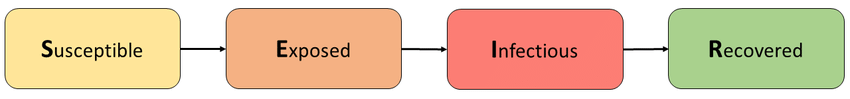
\includegraphics[scale=0.5]{SEIR_einfach}
\caption{SEIR-Modell: Prozedur pro Individuum}
\label{fig:SEIR_einfach}
\end{figure}

Im Weiteren nutzt das Modell ein System aus Differentialgleichungen. Da der Autor noch nicht über das notwendige Wissen verfügt, werden die Gleichungen ohne eine kritische Prüfung übernommen und zur Vollständigkeit dargestellt. Dazu erfolgt eine semantische Einordnung, um im Weiteren, basierend auf den Gleichungen, die Berechnung durchzuführen und die Ergebnisse interpretieren zu können. Die Ausbreitungsdynamik wird im SEIR-Modell durch ein nichtlineares System von „gewöhnlichen Differentialgleichungen“\footnote{Nach \cite{DiffGl} lassen sich viele (biologische) Vorgänge durch solche Gleichungen mathematisch beschreiben.}, siehe Abbildung \ref{fig:Gleichungssystem}, beschrieben.

\begin{figure}[H]
\centering
{
    $s' = -\beta \times S + I$ \\
    $e' = \beta \times S \times I - \alpha \times E$ \\
    $i' = \alpha \times E - \gamma \times I$ \\
    $r' = \gamma \times I$ \\
}
\caption{Gleichungssystem}
\label{fig:Gleichungssystem}
\end{figure}

Die Variablen im ausgeführten Gleichungssystem sind wie folgt semantisch einzuordnen.

\begin{figure}[H]
\centering
\begin{tabular}{ | c | l | }
\hline
 S        & Anteil der Anfälligen \\ 
 E        & Anteil der  der Ausgesetzten \\  
 I        & Anteil der Infizierten \\
 R        & Anteil der Genesenen \\
 $\alpha$ & Übergangsrate (Inkubationszeit) von Ausgesetzten (E) zu Infizierten (I) \\
 $\beta$  & effektive Übertragunsrate (Infektions- oder Transmissionsrate)  \\
 $\gamma$ & Übergangsrate (Erholungszeit) von Infizierten (I) zu Genesenen (G)  \\
\hline
\end{tabular}
\caption{Semantische Bedeutung der Variablen des Gleichungssystem}
\label{fig:SemantikVariablen}
\end{figure}

Anhand der benannten Variablen sind die Gleichungen wie folgt zu verstehen.

\begin{itemize}
    \item \textbf{Gleichung 1:} Diese Gleichung stellt die Veränderungsrate der Individuen vom gesunden zum anfälligen Anteil dar. Das negative Vorzeichen stellt eine negative Veränderung in der gesamten gesunden Bevölkerung dar. Intuitiv ist klar, dass dieser Anteil direkt proportional zur durchschnittlichen Kontaktrate sowie der Gesamtzahl der Infizierten ist.
    \item \textbf{Gleichung 2:} Der erste Term der Gleichung folgt aus der ersten Gleichung, da die Anfälligen in die Kategorie Ausgesetzte wechseln. Der zweite Term repräsentiert die Infizierten.
    \item \textbf{Gleichung 3:} Die Gleichung repräsentiert die Infizierten, diese ergeben sich aus den Ausgesetzten in Abhängigkeit von der Übergangsrate ($\alpha$) abzüglich der Genesenen.
    \item \textbf{Gleichung 4:} Die Gleichung gibt die Zahl der Genesenen in Abhängigkeit der Erholungszeit ($\gamma$) an.
\end{itemize}

Damit sind die Bedeutungen der Gleichungen des SEIR-Modells, soweit nötig und möglich im Rahmen der Arbeit, dargestellt. Wie im Kapitel XY herausgearbeitet spielt der Faktor des „Social Distancing“ bei einer pandemischen Lage, insbesondere bei hochansteckenden (Bronchial-) Viren wie Covid-19, eine zentrale Rolle. Aus diesem Grund wird das Modell um einen Faktor erweitert. Die ersten beiden Gleichungen des Systems werden um den Parameter 'rho' ($\rho$) ergänzt, damit ergeben sich folgende Gleichungen.

\begin{itemize}
    \item $s' = -(1-\rho)*\beta*S+I$
    \item $e' = (1-\rho)*\beta*S*I-\alpha*E$
\end{itemize}

Der Parameter '$\rho$' wird als Anteil im Wertebereich von 0 bis 1 angegeben. Lockdowns und andere öffentliche (Ausgangs-) Beschränkungen resultieren in einem hohen Wert für $\rho$. Vollständiges Social Distancing entspricht $\rho$ = 1 und würde dazu führen, dass sich keine weiteren gesunden Personen infizieren.\footnote{Die Erweiterung des Systems durch den Paramter $\rho$ erfolgt wiederum in vereinfachter Form, eine ausführliche wissenschaftliche Darlegung erfolgt bspw. in einem Artikel im Nature erschien, siehe \cite{EffectSocDist}.}

Aufbauend auf dem Gleichungssystem und dem semantischen Verständnis des erweiterten SEIR-Modells kann nun die programmatische Umsetzung erfolgen.

\subsection{Umsetzung}
Die Umsetzung erfordert zunächst die Abbildung des erweiterten Modells in Form von Gleichungen in Quellcode. Dazu werden Funktionen erstellt, die es ermöglichen die benannten Parameter beliebig zu ändern, die Simulation zu starten und anschließend auszuwerten.

\subsubsection{Abbildung des Modells in Python}
Das dargestellte erweiterte Modell lässt sich ohne große Schwierigkeiten geradlinig in Python übertragen und implementieren, das folgende Codelisting \ref{StartFunktion} zeigt die Implementierung der Berechnung in der Funktion 'start'. Die vollständige Implementierung in einer Python-Klasse inklusive Kommentare zur Dokumentation und zum Verständnis befindet sich im Anhang (Kapitel \ref{sec:Anhang} ab Seite \pageref{sec:Anhang}). Die funktionale Implementierung beläuft sich auf nur ca. 130 Codezeilen. Dabei spielt wiederum Python seine Stärke aus, da nur minimaler „Boilerplate Code“\footnote{Damit wird Code bezeichnet der nicht unmittelbar zur Funktionalität beiträgt, sondern durch die Syntax der Sprache notwendig ist.} notwendig ist.

\lstinputlisting[language=Python, caption=Python-Umsetzung zur Berechnung in der Funktion 'start', label=StartFunktion]{SEIR_Simulation_run.py}

\subsection{Berechnung und grafische Darstellung}
Um die Mächtigkeit einer, wenn auch vereinfachten Simulation, hier darzustellen werden im Folgenden durch den Autor verschiedene Szenarien beschrieben, simuliert und im Kontext interpretiert. Jedes Szenario wird kurz erläutert und die semantisch zugehörigen Parameter quantifiziert. Der Ausgangspunkt aller Szenarien ist eine nahezu 100\% gesunde Bevölkerung („Anfällige“), in der zu Beginn nur 0,001\% dem Virus ausgesetzt waren. Wird für Deutschland eine Bevölkerung von 83 Mio. angenommen, sind am Anfang der Simulation 830 Menschen dem Virus ausgesetzt gewesen.

\subsubsection{Szenario 1 - „Covid-19“}
Das erste Szenario soll eine ähnliche Situation darstellen, wie zu Beginn der Covid-19 Pandemie.\footnote{Die Parameter basieren auf Veröffentlichungen des RKI vom März 2020, siehe \cite{SEIRParameter}.} Die durchschnittliche Übertragungsrate ($\beta$) lag zu Beginn der Pandemie bei etwas unter 2 und es gab noch keine Kontaktbegrenzungen. Vor der Simulation erfolgt die Initialisierung der Parameter, siehe Listing \ref{Szenario1}.

\begin{lstlisting}[language=Bash, caption=Szenario 1 - Covid-19, label=Szenario1]
bash-3.2$ python3
Python 3.8.9 (default, Oct 26 2021, 07:25:54) 
[Clang 13.0.0 (clang-1300.0.29.30)] on darwin
Type "help", "copyright", "credits" or "license" for more information.
>>> import SEIR_Simulation as s
>>> modell = s.SEIR()
>>> modell.setze_parameter(parameter_=[0.2, 1.75, 0.5, 0.1], verbose=True)
Setzen der Parameter mit den folgenden Werten:
--------------------------------------------------
alpha (Inkubationszeit):    0.2
beta  (Uebertragunsrate):   1.75
gamma (Erholungszeit):      0.5
rho   (Social Distancing):  0.1
>>> diagramm = modell.start(zeit_max=90, zeit_intervall=0.01)
>>> modell.zeichnen(diagramm, tage=90)
\end{lstlisting}

Die Umgebung (Python) wird dazu gestartet (Zeile 1) und die Klasse importiert (Zeile 5). Nach dem Import kann die Klasse verwendet und ein Objekt der Klasse instanziiert werden (Zeile 6). Im nächsten Schritt werden die Parameter gesetzt (Zeile 7) und durch Nutzung des Arguments 'verbose'\footnote{Wörtlich übersetzt heißt es wortreich/langatmig.} zur Kontrolle ausgegeben (Zeile 7 - 13). Nachdem alle Parameter gesetzt sind wird die Berechnung durch Aufruf der Funktion 'start', mit den Parametern zu Dauer und Intervall, ausgeführt. Als letztes wird die Berechnung der Funktion 'zeichnen' übergeben und ausgegeben, das Ergebnis zeigt Abbildung \ref{fig:szenario_1}

\begin{figure}[H]
\centering
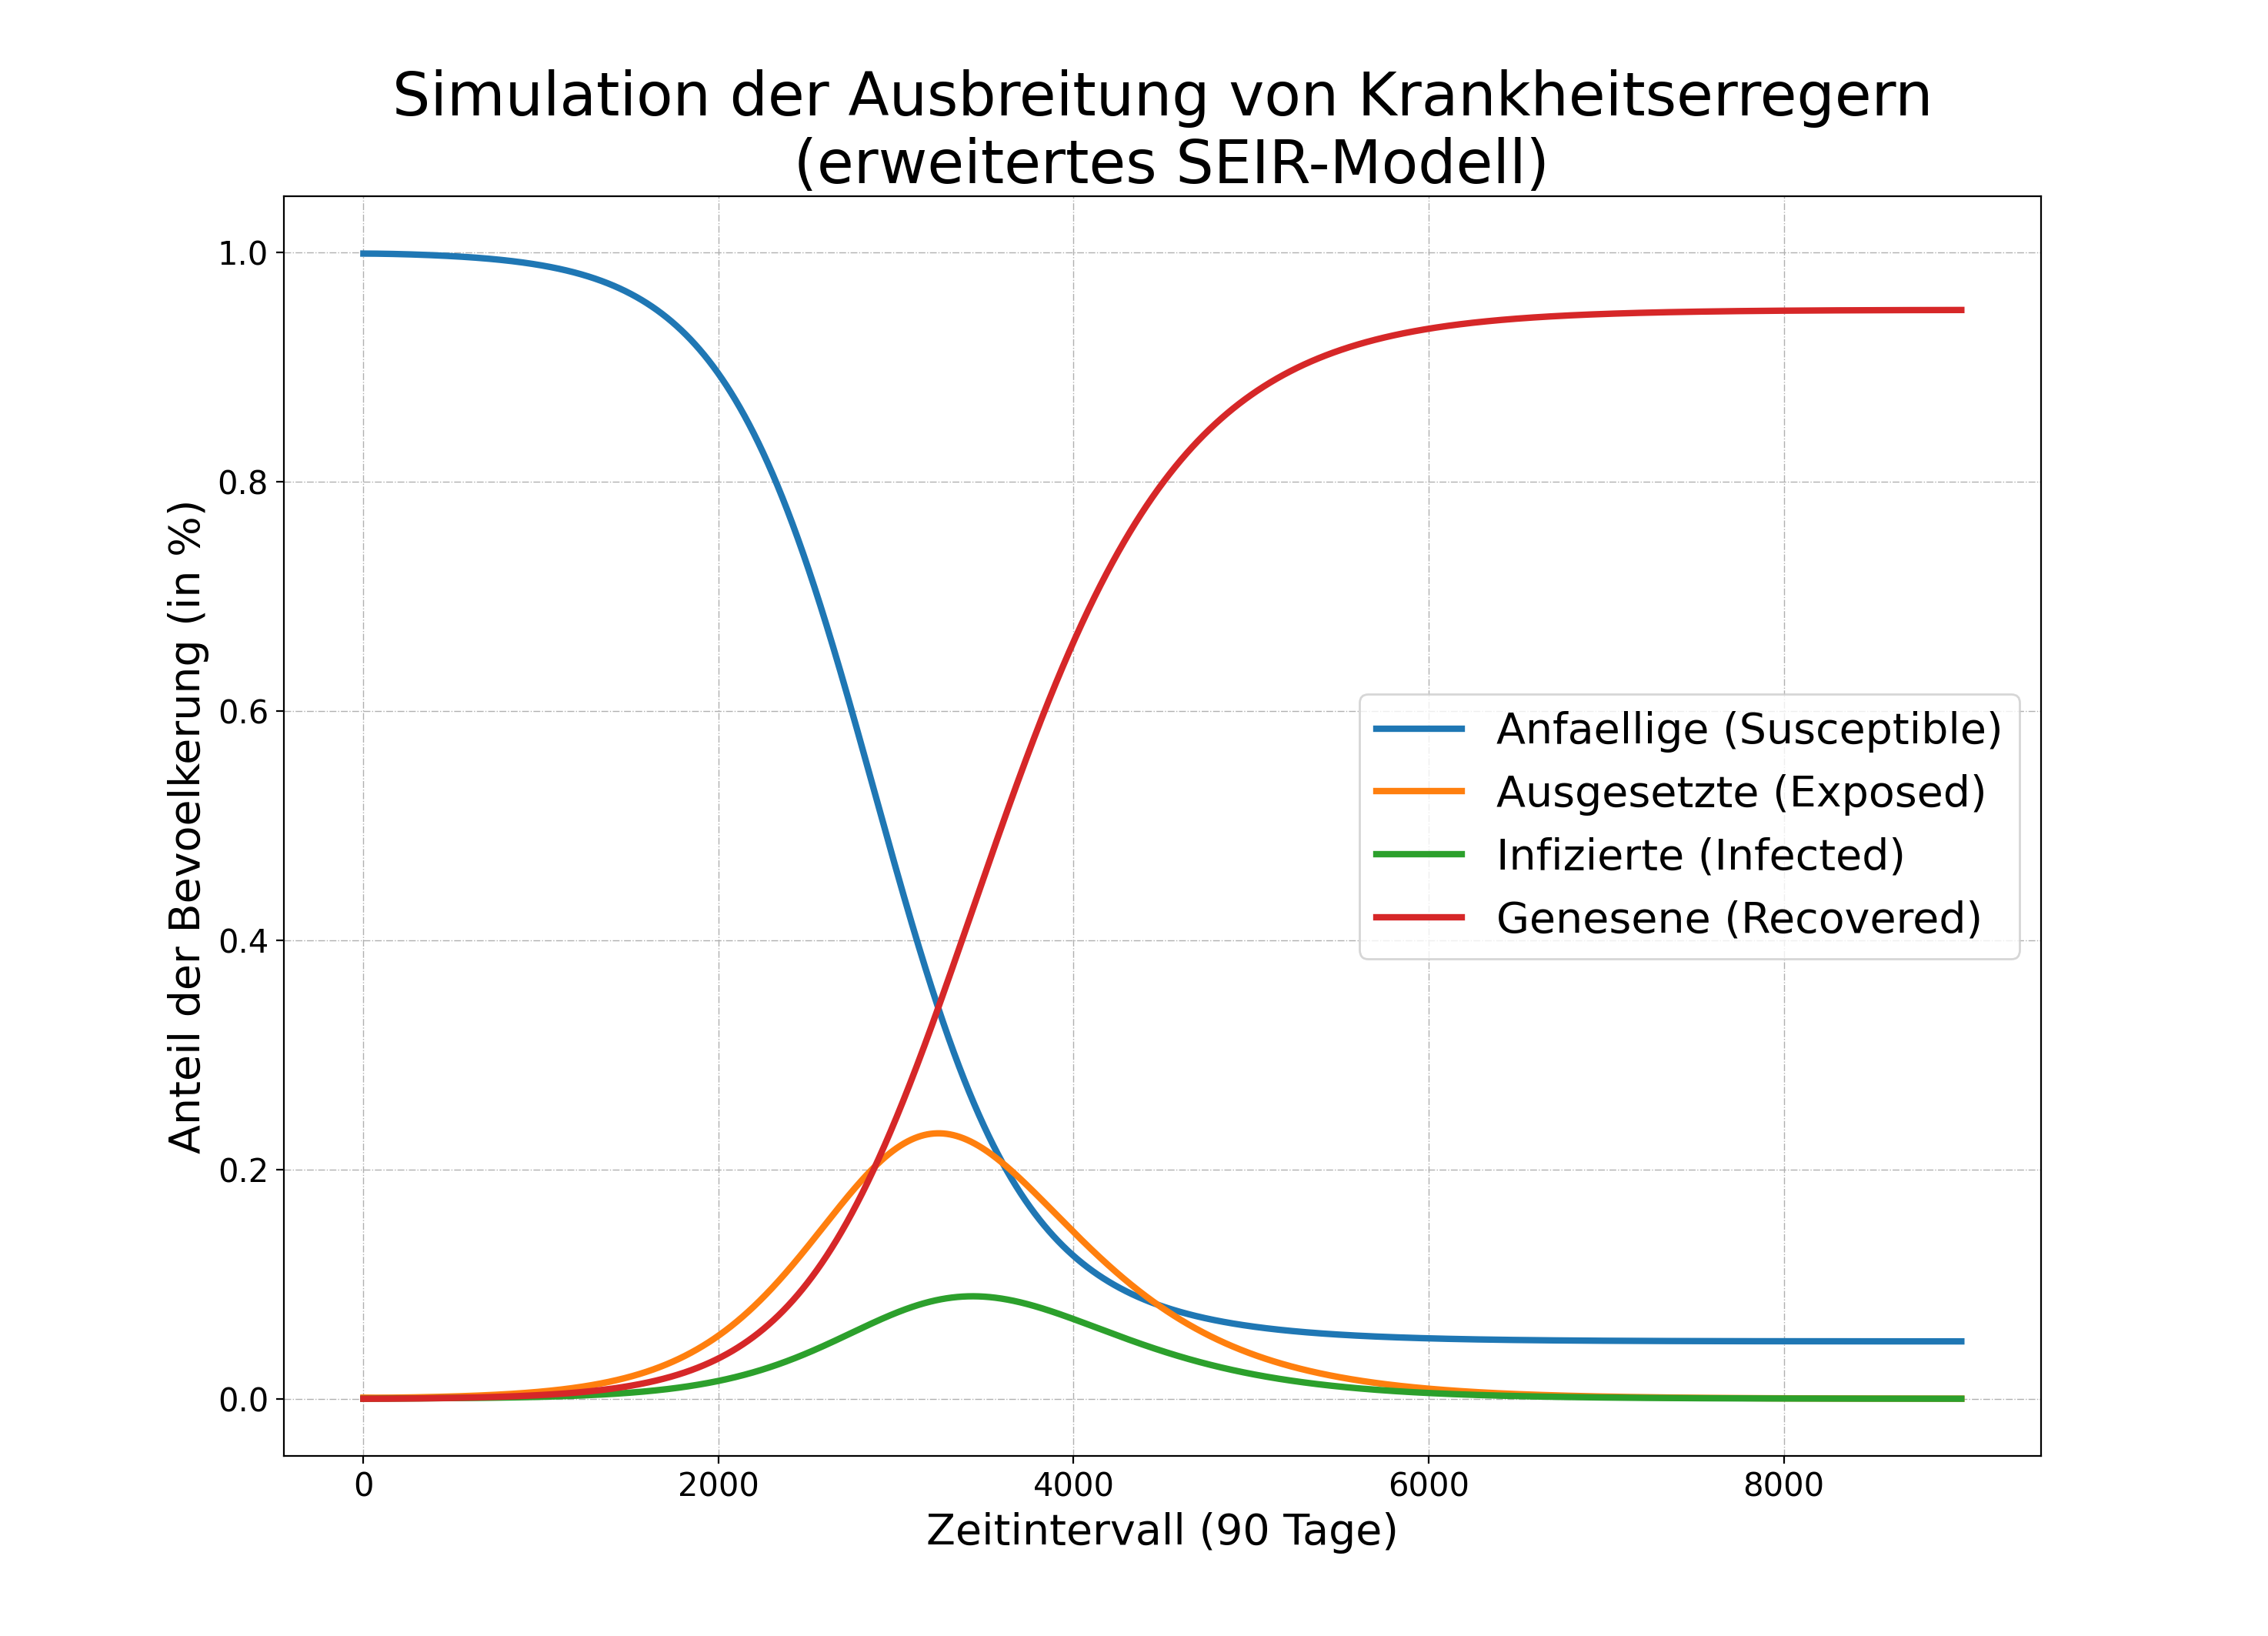
\includegraphics[scale=0.4]{Szenario_1}
\caption{Szenario 1}
\label{fig:szenario_1}
\end{figure}

\paragraph{Szenario 1.1 - Covid-19 mit höherer Übertragungsrate}
In Kapitel „\ref{subsec:Cov-Ausbreitung} \nameref{subsec:Cov-Ausbreitung}“ wird im November 2021, infolge von Virusmutationen, eine höhere Übertragungsrate (2,8 bis 3,8) festgestellt. Für die Simulation wird für $\beta$ ein Wert von 3,0 angenommen, siehe Zeile 5 im Listing \ref{lst:Szenario1_beta3}. Die Simulation wurde auf 70 Tage begrenzt, da ein noch drastischerer Verlauf erwartbar und in Abbildung \ref{fig:Szenario_1_beta30} deutlich erkennbar ist.

\begin{lstlisting}[language=Bash, caption=Szenario 1 - Covid-19 (hohe Übertragungsrate)), label=lst:Szenario1_beta3]
modell.setze_parameter(parameter_=[0.2, 3.00, 0.5, 0.1], verbose=True)
Setzen der Parameter mit den folgenden Werten:
--------------------------------------------------
alpha (Inkubationszeit):    0.2
beta  (Uebertragunsrate):   3.0
gamma (Erholungszeit):      0.5
rho   (Social Distancing):  0.1
>>> diagramm = modell.start(zeit_max=70, zeit_intervall=0.1)
>>> modell.zeichnen(diagramm, tage=70)
\end{lstlisting}

\begin{figure}[H]
\centering
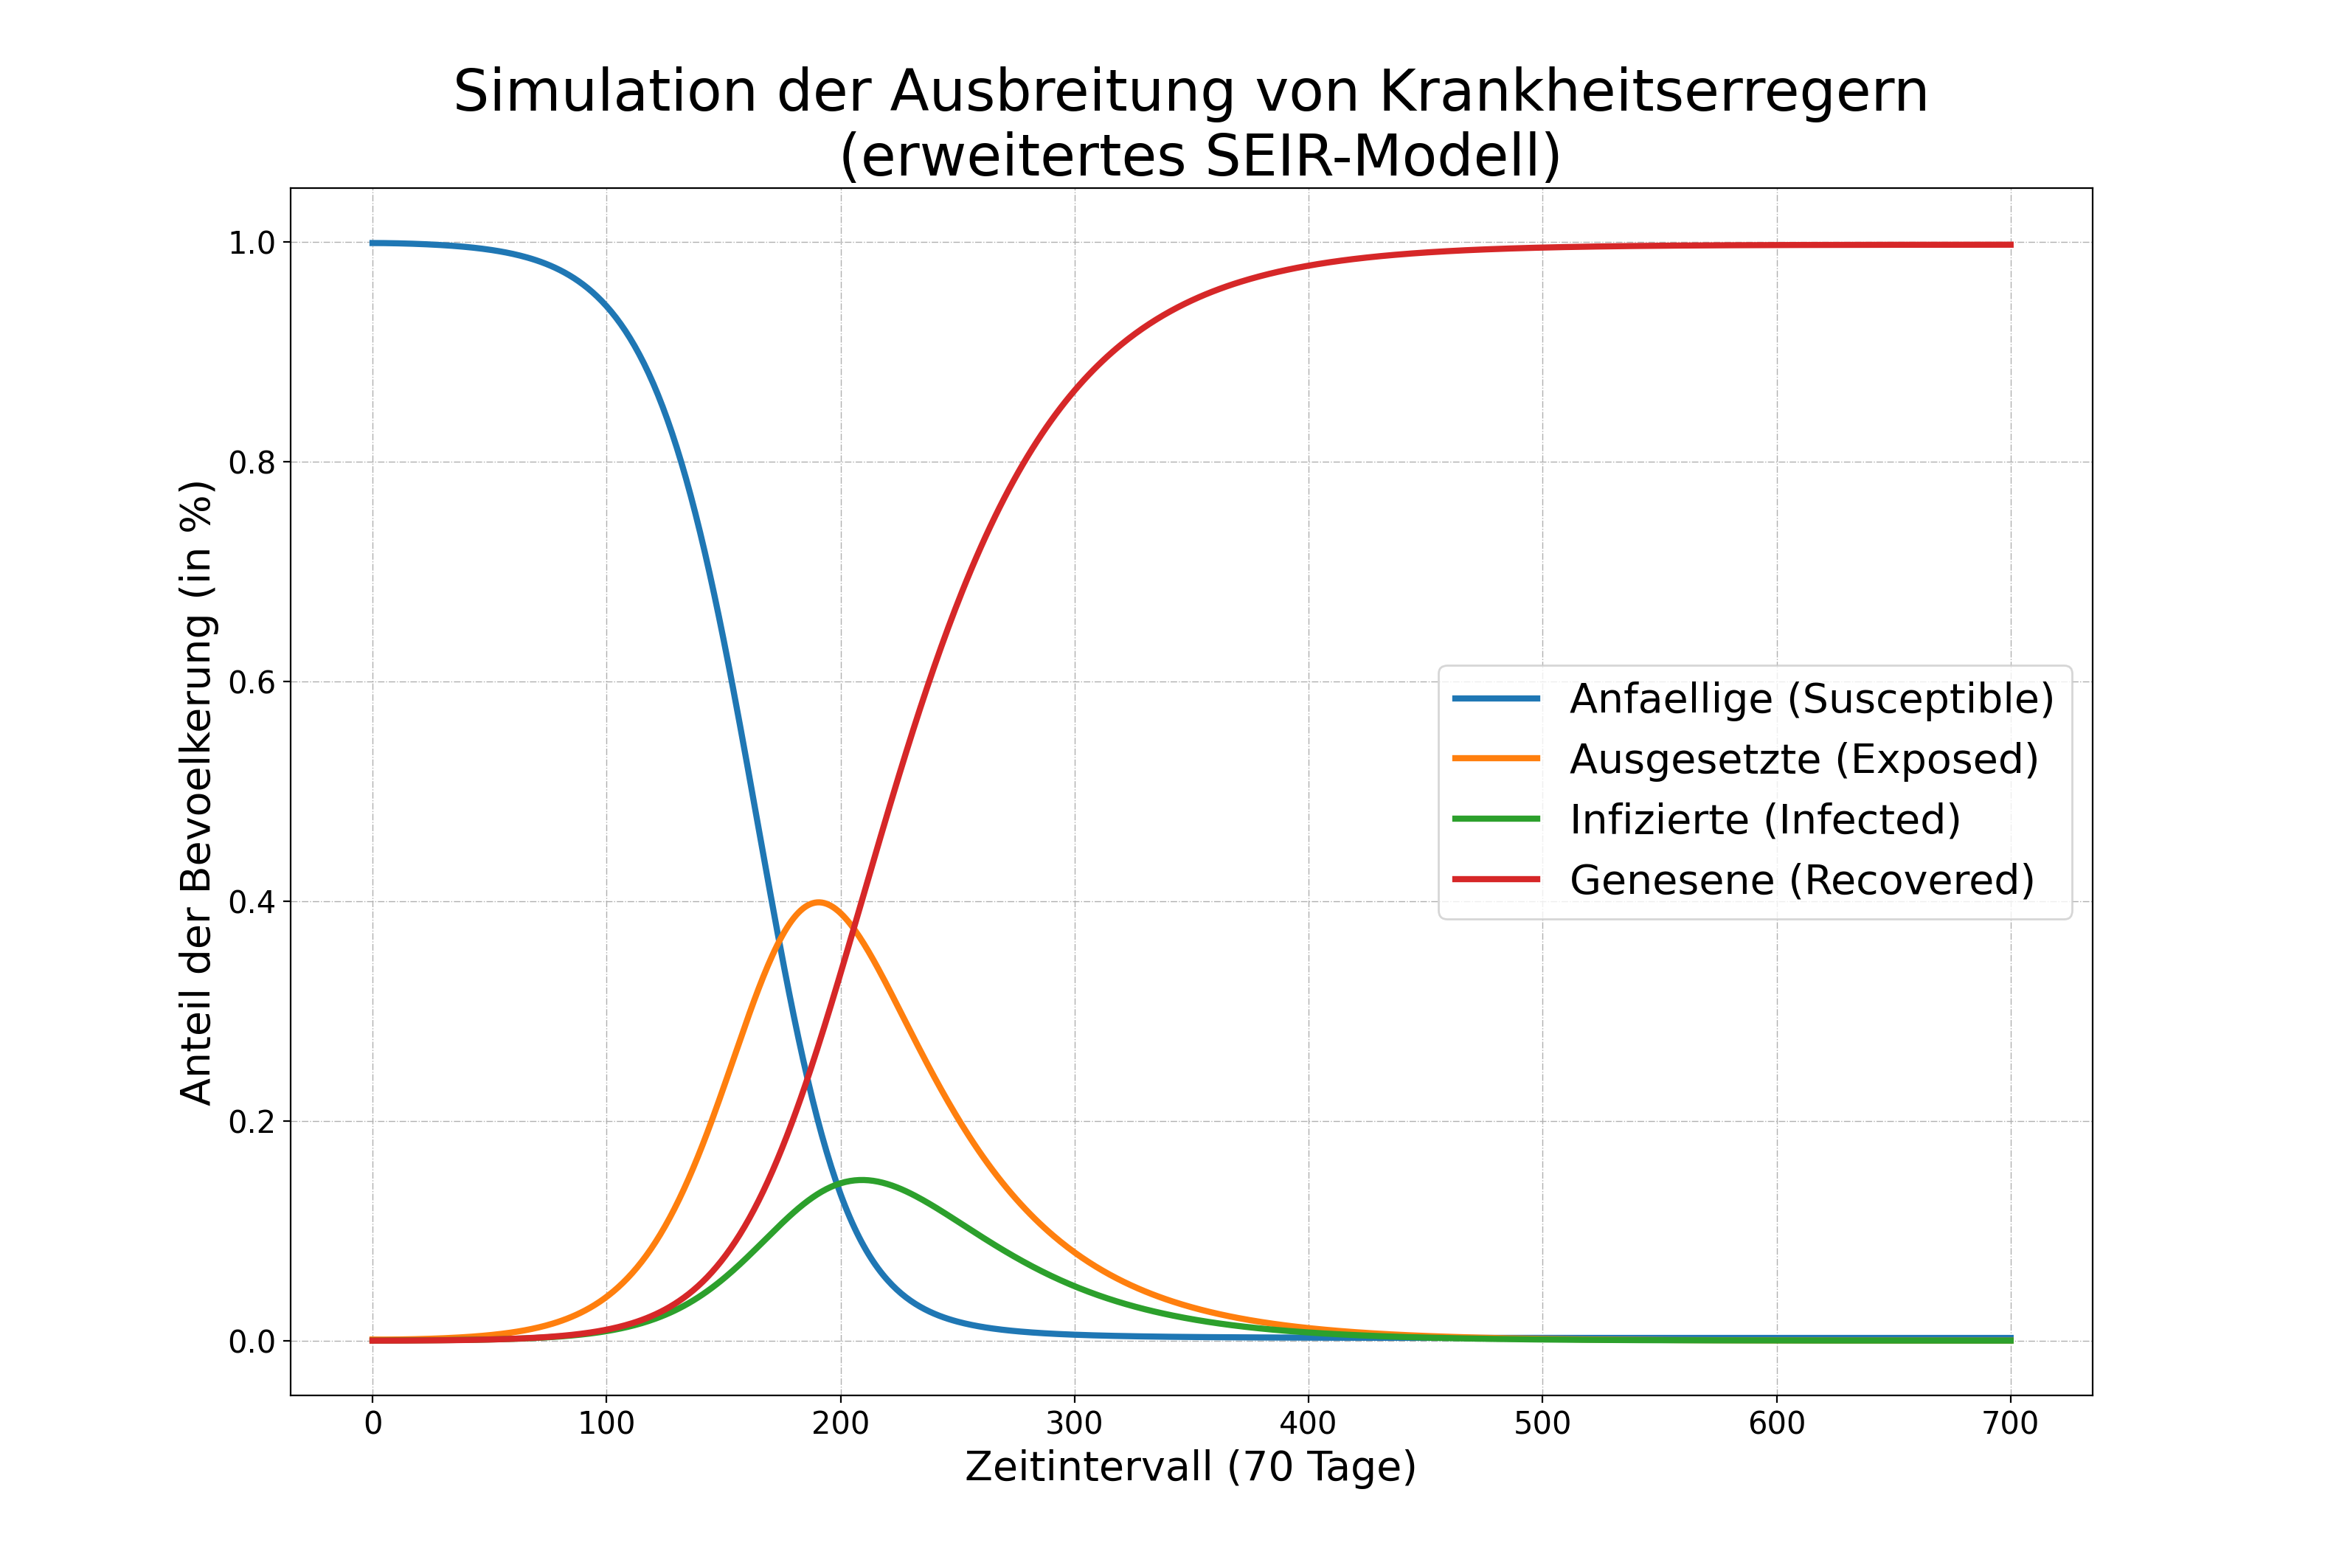
\includegraphics[scale=0.35]{Szenario_1_beta30}
\caption{Szenario 1.1 mit höherer Übertragungsrate ($\beta$=3)}
\label{fig:Szenario_1_beta30}
\end{figure}


\paragraph{Einordnung Szenario 1}
Schon dieses einfache Szenario zeigt wie rapide sich ein Virus in einer Population ausbreiten kann, wenn keine Maßnahmen getroffen werden. Bereits nach weniger als der Hälfte der 90 Tage-Simulation wären etwa 22\% dem Virus ausgesetzt und knapp 10\% zeigen Symptome und sind somit infiziert. Für Deutschland wären zu diesem Zeitpunkt also ca. 18 Mio. Menschen ausgesetzt (also potentiell positiv) und ca. 8.3 Mio. Menschen nachweisbar positiv gewesen. In Kapitel „\ref{subsec:Cov-Verlauf} \nameref{subsec:Cov-Verlauf}“ werden 19\% der Infektionen mit einem schweren Verlauf und 1,7\% mit tödlichem Verlauf ausgewiesen. Im Resultat hätten zum Höhepunkt der Pandemie ca. 1,57 Mio. Menschen mit einem schweren Verlauf zu kämpfen und 141.000 Menschen wären (innerhalb weniger Tage) gestorben. Ein solches Infektionsgeschehen hätte mit an Sicherheit grenzender Wahrscheinlichkeit zu einem totalen Kollaps in Deutschland geführt. Ein direkter Vergleich mit den Todeszahlen des RKI, die für das Jahr 2020 41.476 Todesfälle ausweisen, zeigt die Wirksamkeit der drastischen Maßnahmen.\footnote{Vgl. \url{https://www.tagesschau.de/inland/corona-tote-107.html}}

Die Kurven im angepassten Szenario 1.1 zeigen, wie zu erwarten, einen noch höheren Verlauf des Infektionsgeschehens. Dabei muss in die Auswertung einbezogen werden, dass die erhöhte Übertragungsrate mit anderen Auswirkungen, weniger schwere Verläufe und Todesfällle, einhergeht.

\subsubsection{Szenario 2 - Auswirkung von Social Distancing}
Bei neu auftretenden Krankheiten ist in der Regel nicht sofort die notwendige Medizin oder Impfung verfügbar. Um ein Kollaps, siehe Szenario 1 in Abbildung \ref{fig:szenario_1}, zu vermeiden ist der entscheidende Faktor die Vereinzelung bzw. die Reduktion von Kontakten und Reisen um das Verbreiten des Virus zu unterbinden. Dazu wird im Folgenden der Social Distancing-Faktor in drei Stufen (0.2, 0.4 und 0.6) verändert (siehe Listing \ref{lst:Szenario2}, jeweils die Simulation berechnet und anschließend wiederum im Kontext eingeordnet.

\begin{lstlisting}[language=Bash, caption=Szenario 2 - Social Distancing, label=lst:Szenario2]
>>> modell.setze_parameter(parameter_=[0.2, 1.75, 0.5, 0.2], verbose=True)
Setzen der Parameter mit den folgenden Werten:
--------------------------------------------------
alpha (Inkubationszeit):    0.2
beta  (Uebertragunsrate):   1.75
gamma (Erholungszeit):      0.5
rho   (Social Distancing):  0.2
>>> diagramm = modell.start(zeit_max=90, zeit_intervall=0.01)
>>> modell.setze_parameter(parameter_=[0.2, 1.75, 0.5, 0.4], verbose=True)
Setzen der Parameter mit den folgenden Werten:
--------------------------------------------------
alpha (Inkubationszeit):    0.2
beta  (Uebertragunsrate):   1.75
gamma (Erholungszeit):      0.5
rho   (Social Distancing):  0.4
>>> diagramm = modell.start(zeit_max=90, zeit_intervall=0.01)
>>> modell.zeichnen(diagramm, tage=90)
>>> modell.setze_parameter(parameter_=[0.2, 1.75, 0.5, 0.6], verbose=True)
Setzen der Parameter mit den folgenden Werten:
--------------------------------------------------
alpha (Inkubationszeit):    0.2
beta  (Uebertragunsrate):   1.75
gamma (Erholungszeit):      0.5
rho   (Social Distancing):  0.6
>>> diagramm = modell.start(zeit_max=190, zeit_intervall=0.01)
>>> modell.zeichnen(diagramm, tage=190)
\end{lstlisting}

\begin{figure}[H]
\centering
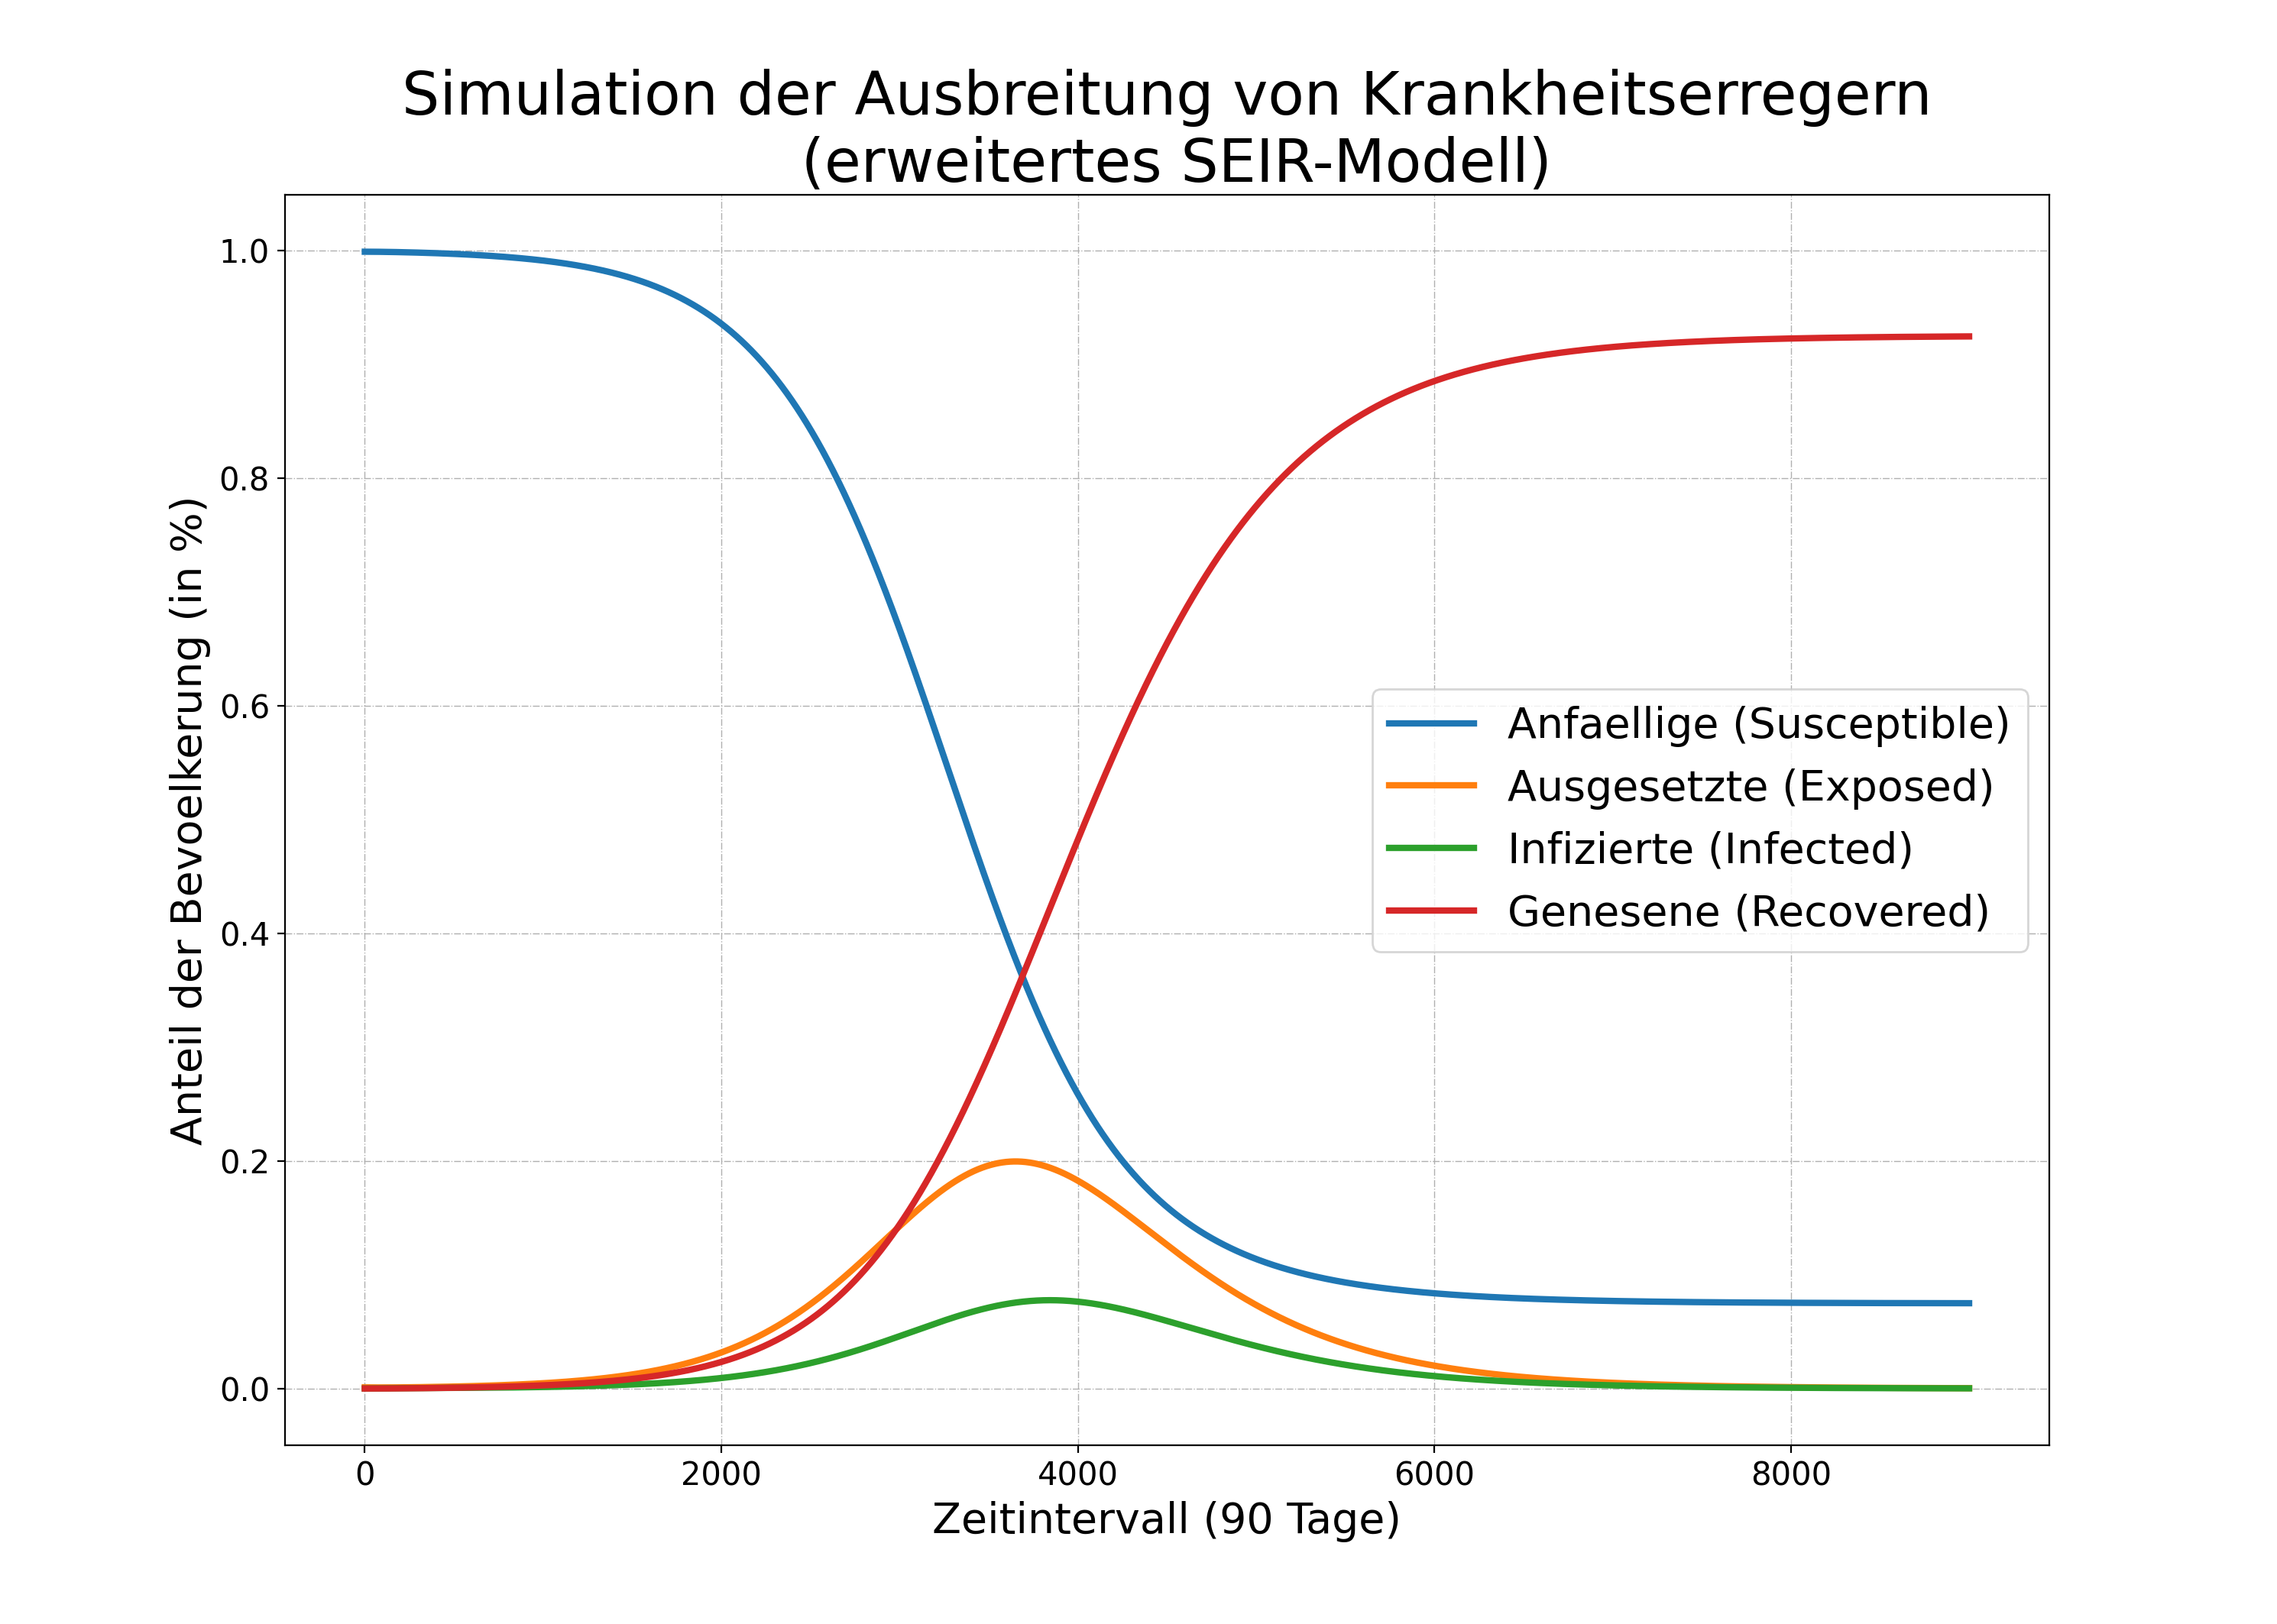
\includegraphics[scale=0.4]{Szenario_2_rho_0.2}
\caption{Szenario 2 - $\rho$=0.2}
\label{fig:szenario_2_0.2}
\end{figure}

\begin{figure}[H]
\centering
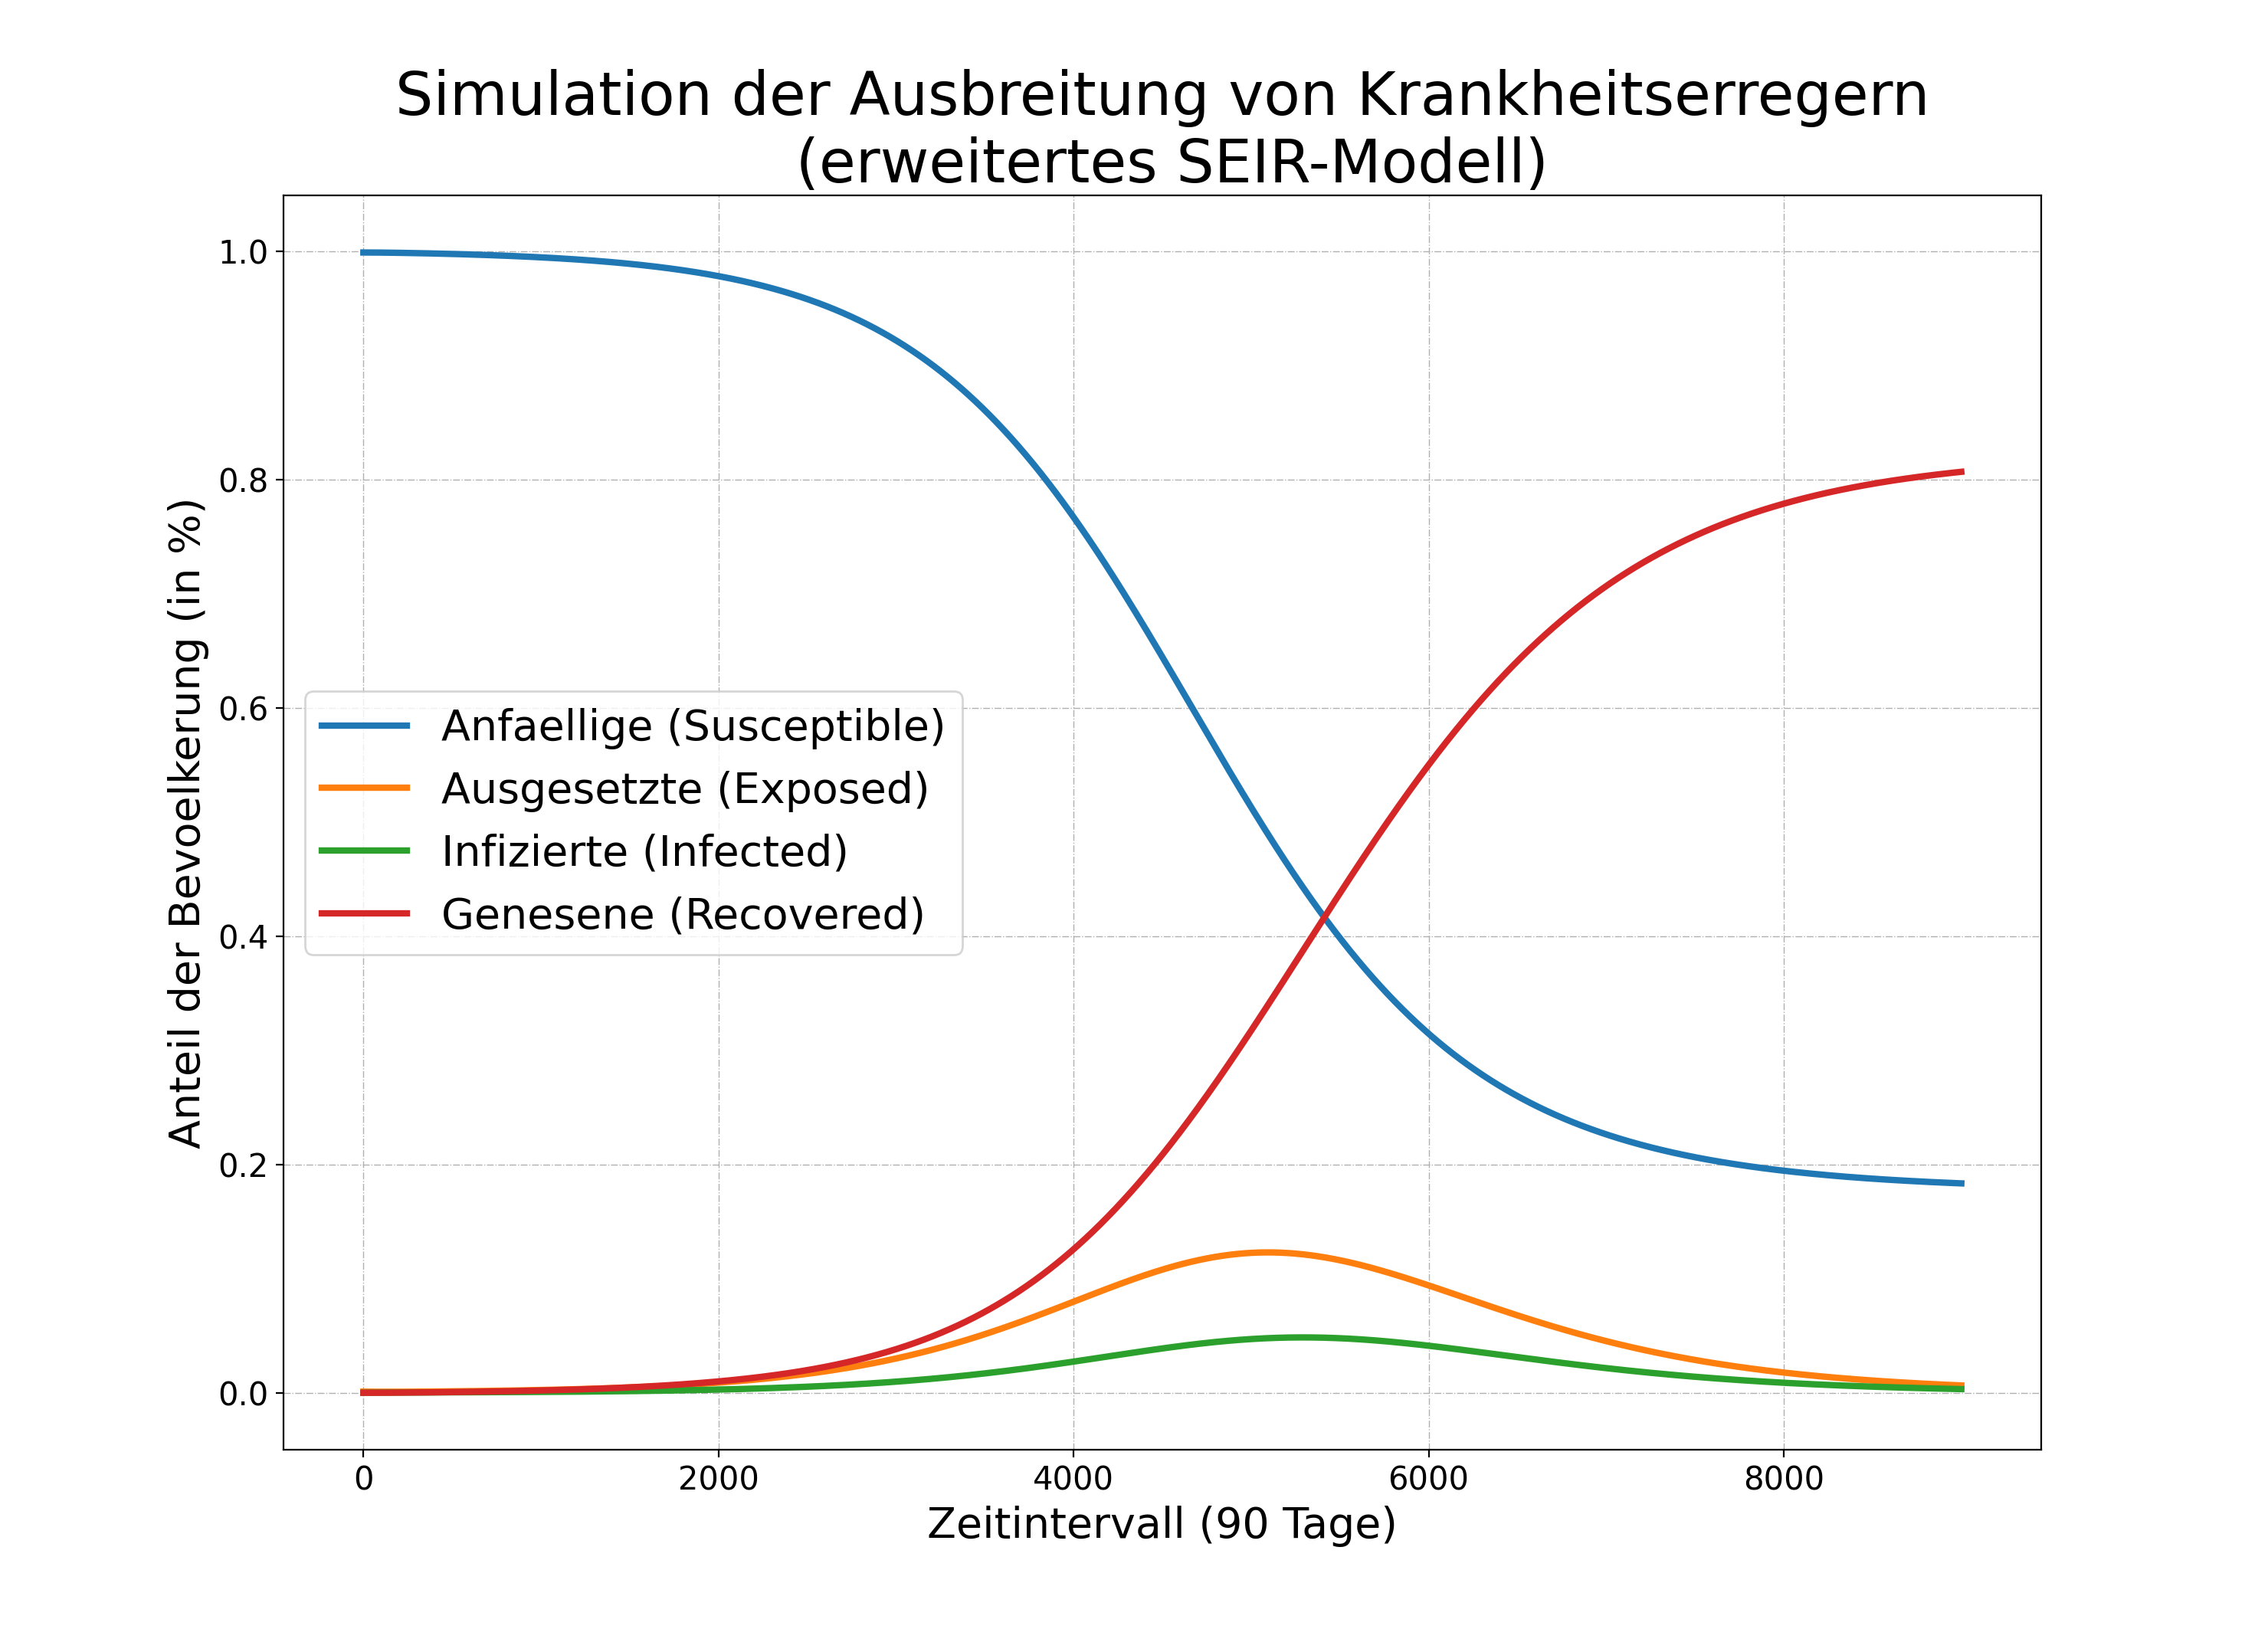
\includegraphics[scale=0.4]{Szenario_2_rho_0.4}
\caption{Szenario 2 - $\rho$=0.4}
\label{fig:szenario_2_0.4}
\end{figure}

\begin{figure}[H]
\centering
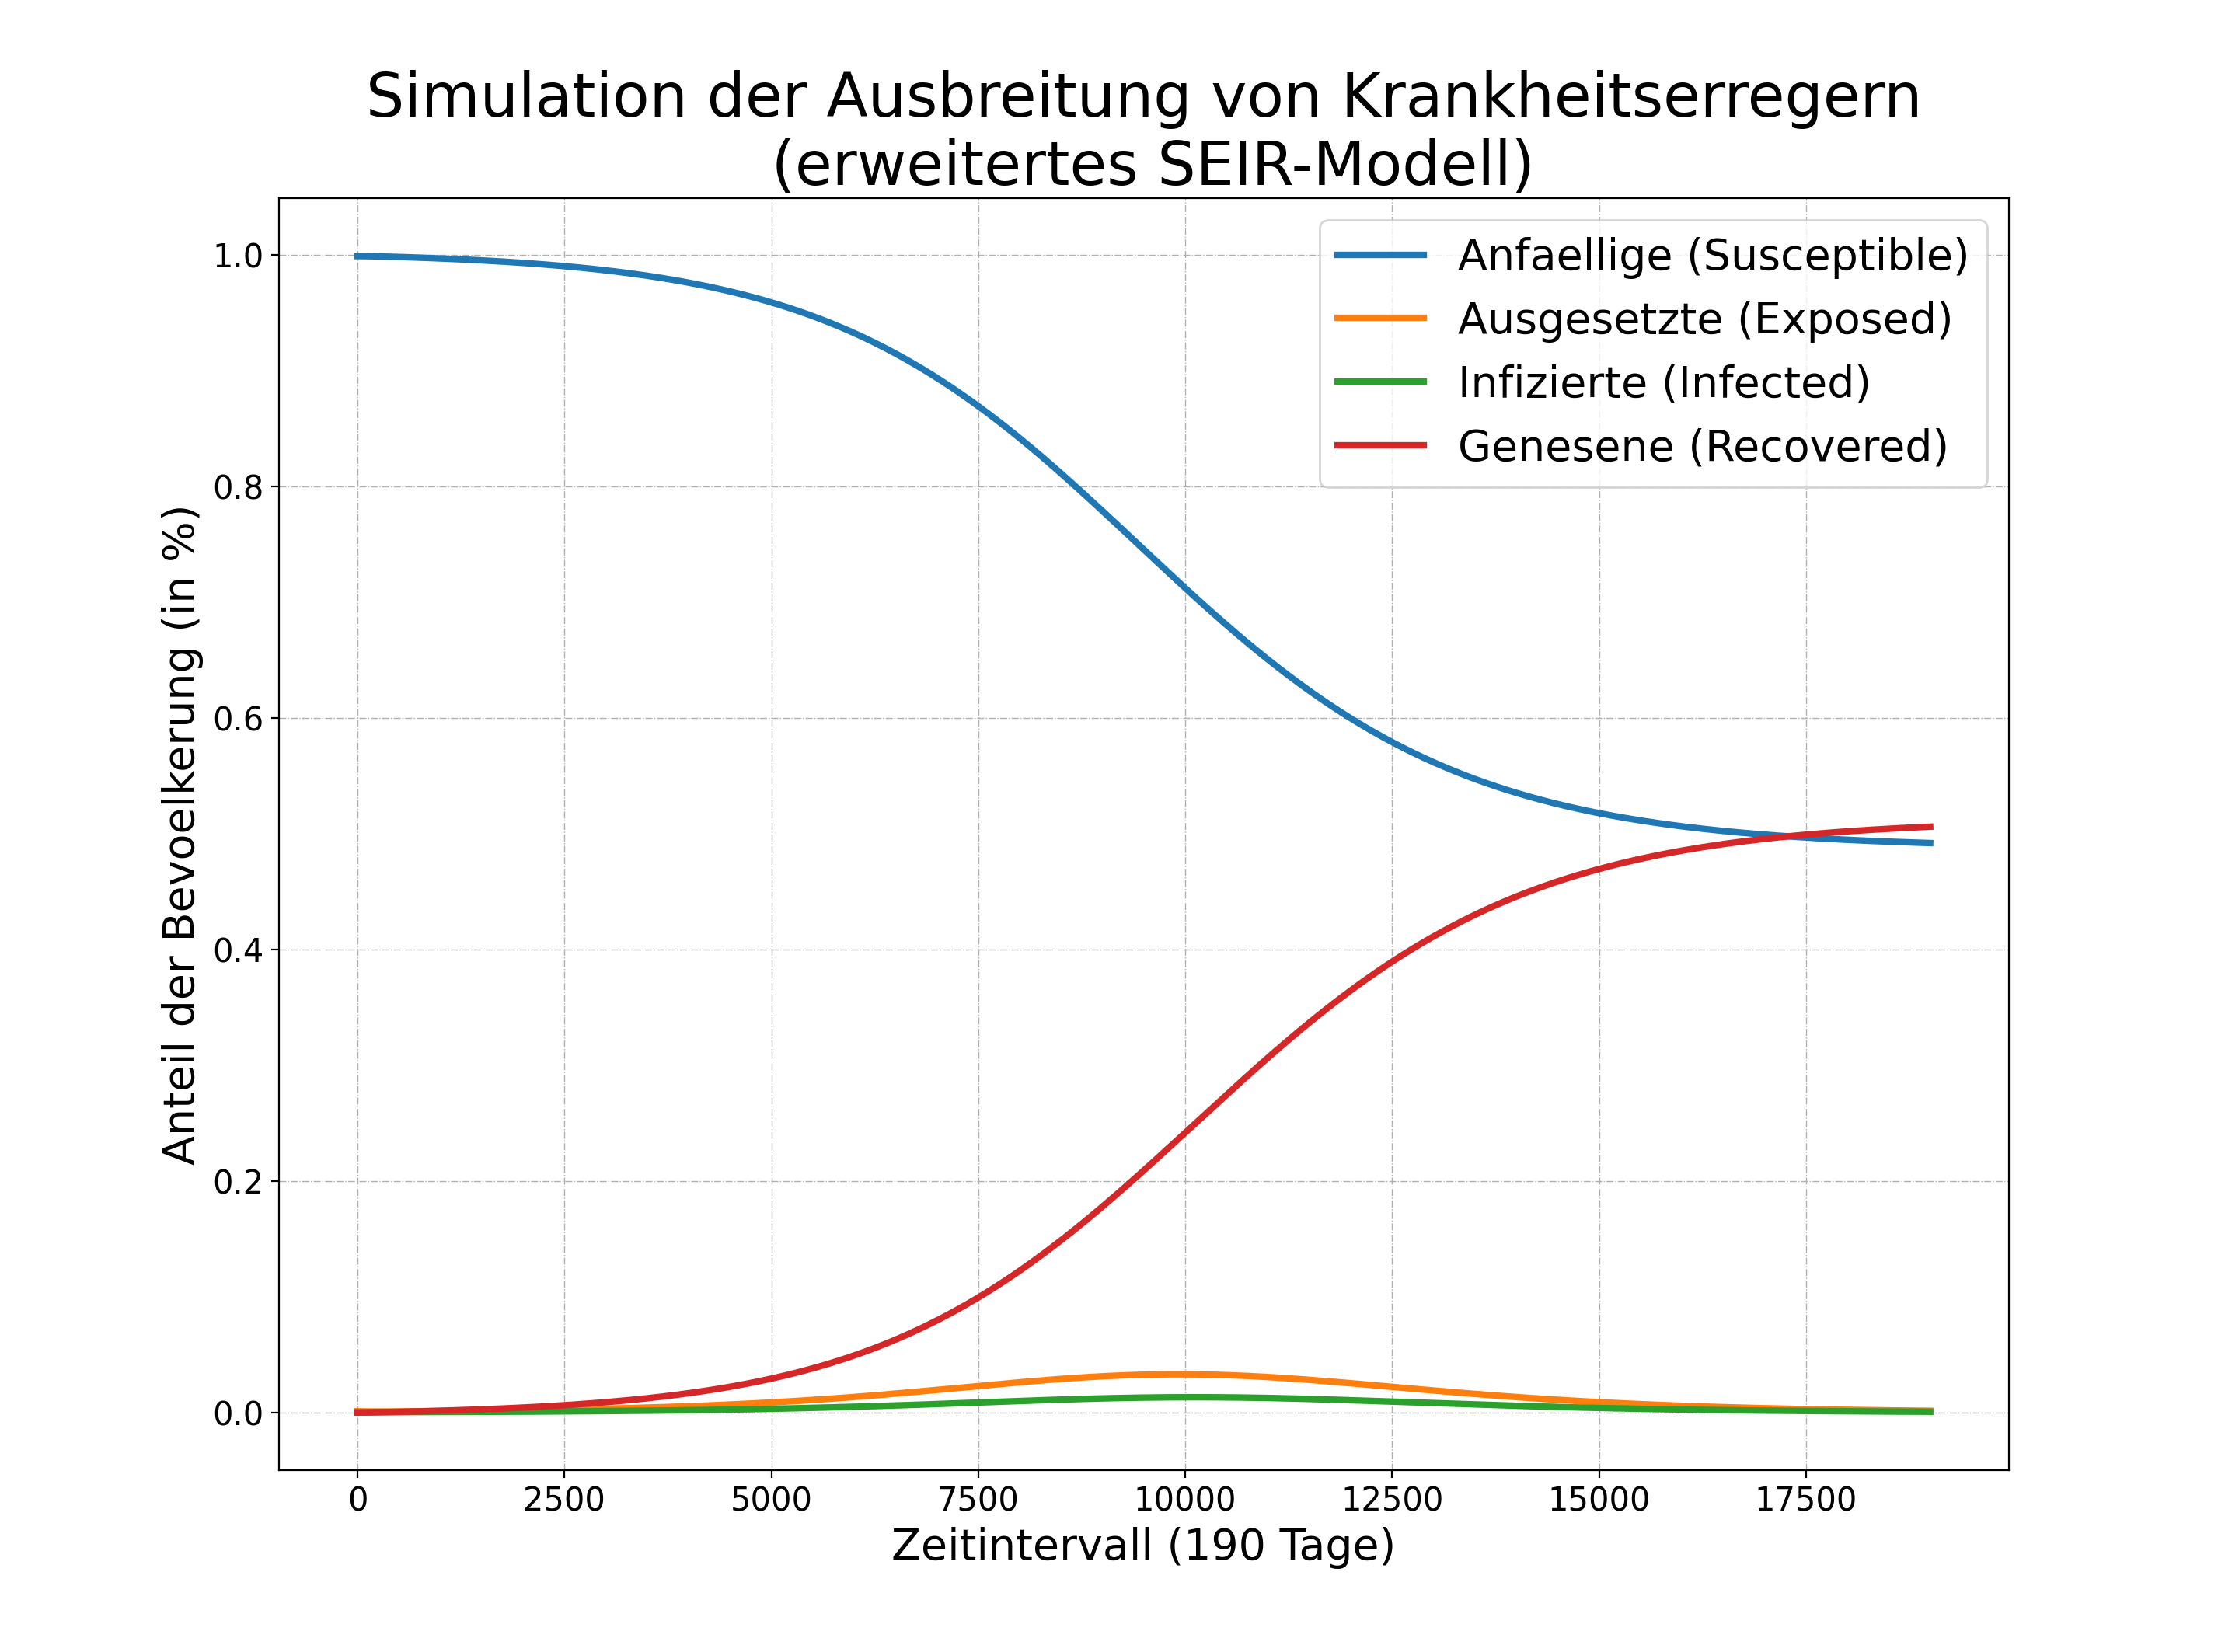
\includegraphics[scale=0.4]{Szenario_2_rho_0.6}
\caption{Szenario 2 - $\rho$=0.6}
\label{fig:szenario_2_0.6}
\end{figure}

\paragraph{Einordnung Szenario 2 - „Social Distancing“}
Die Abbildungen \ref{fig:szenario_2_0.2}, \ref{fig:szenario_2_0.4} und \ref{fig:szenario_2_0.6} zeigen auf den ersten Blick den, im Sinne der Verminderung von Infektionen, positiven Effekt von Social Distancing. Eine minimale Einschränkung der Bewegung im öffentlichen Raum ($\rho$=0,2) zeigt nur einen kleinen Effekt, aber schon ein Faktor von $\rho$=0,4, siehe Abbildung \ref{fig:szenario_2_0.4}, also eine Verringerung der Kontaktrate um 40\%, durch Maßnahmen wie Home Office und Masken tragen, zeigt Wirkung in Form einer deutlich flacheren Kurve. Auch zu sehen ist jedoch, dass die Infektionszahlen immer noch zu einem Kollaps des Gemein- und Sozialwesens führen würde. Erst mit einer deutlichen Verringerung der Kontaktrate von mehr als 50\%, in Abbildung \ref{fig:szenario_2_0.6} mit $\rho$=0,6 simuliert, wird die Infektionskurve signifikant flacher. Unmittelbar erkennbar ist der deutlich längere Verlauf der Pandemie. Aus diesem Grund wurde die Simulation auf 190 Tage verlängert (Listing \ref{lst:Szenario2} - Zeile 25), sowie die Stagnation des Anteils der Genesenen. Damit sind verschiedene Probleme ableitbar. Die Dauer der notwendigen Einschränkungen der Freiheit ist der Bevölkerung nicht zumutbar. Zudem stößt das Modell an seine Grenzen, gegen Ende der Simulation stagniert die Zahl der Genesenen und Anfälligen bei jeweils ca. 50\% der Population. In einer realen Umgebung ist davon auszugehen, dass es weiterhin Infektionen gibt, jedoch wäre der Zeitrahmen bis zum Erreichen der endemischen Lage sehr lang.

\subsubsection{Szenario 3 - Aufhebung eines Lockdown}
Das dritte Szenario leitet sich aus den vorhergehenden Szenarien unmittelbar ab. Eine Pandemie ohne soziale Restriktionen führt zum Kollaps der Gesellschaft. Ebenso nicht umsetzbar ist ein dauerhafter Lockdown bzw. signifikante Einschränkungen des gesellschaftlichen Lebens. Daraus ergibt sich eine Verknüpfung von Lockerungen und Verschärfungen der Restriktionen. Dieses Szenario soll die Entwicklung beim Übergang von einem Lockdown zu Lockerungen und umgekehrt simulieren. Im Listing \ref{lst:Szenario3} wird zunächst das Modell mit hohem Lockdown-Faktor ($\rho$=0,6) initialisiert (Zeile 3) und die Entwicklung für 100 Tage simuliert. Das Ergebnis wird in der Variable 'result1' gespeichert (Zeile 10). Anschließend wird ein zweites Modell mit den Werten vom ersten Modell initialisiert (Zeile 11 - 12). Für Modell 2 wird der Social Distancing Faktor für die Lockerung auf 0.1 angepasst (Zeile 13). Zum Schluss werden die beiden Ergebnisse mit der Numpy-Funktion 'vstack' in ein Array vereint und mit Hilfe der Funktionen 'zeichnen' und 'zeichne\_variable' (Zeile 22 - 23) ausgegeben, siehe Abbildung \ref{fig:szenario_3} und \ref{fig:szenario_3_Infizierte}.

\begin{lstlisting}[language=Bash, caption=Szenario 3 - Aufhebung eines Lockdown, label=lst:Szenario3]
>>> import numpy as np
>>> modell = s.SEIR()
>>> modell.setze_parameter(parameter_=[0.2, 1.75, 0.5, 0.6], verbose=True)
Setzen der Parameter mit den folgenden Werten:
--------------------------------------------------
alpha (Inkubationszeit):    0.2
beta  (Uebertragunsrate):   1.75
gamma (Erholungszeit):      0.5
rho   (Social Distancing):  0.6
>>> result1 = modell.start(zeit_max=100, zeit_intervall=0.1)
>>> neu_init = modell.vals_
>>> modell2 = s.SEIR(initiale_werte=neu_init)
>>> modell2.setze_parameter(parameter_=[0.2, 1.75, 0.5, 0.1], verbose=True)
Setzen der Parameter mit den folgenden Werten:
--------------------------------------------------
alpha (Inkubationszeit):    0.2
beta  (Uebertragunsrate):   1.75
gamma (Erholungszeit):      0.5
rho   (Social Distancing):  0.1
>>> result2 = modell2.start(zeit_max=120, zeit_intervall=0.1, zuruecksetzen=False)
>>> result3 = np.vstack((result1,result2))
>>> modell2.zeichnen(result3, tage=220)
>>> modell2.zeichnen_variable(result3[:,2], var_name='Infizierte')
\end{lstlisting}

\begin{figure}[H]
\centering
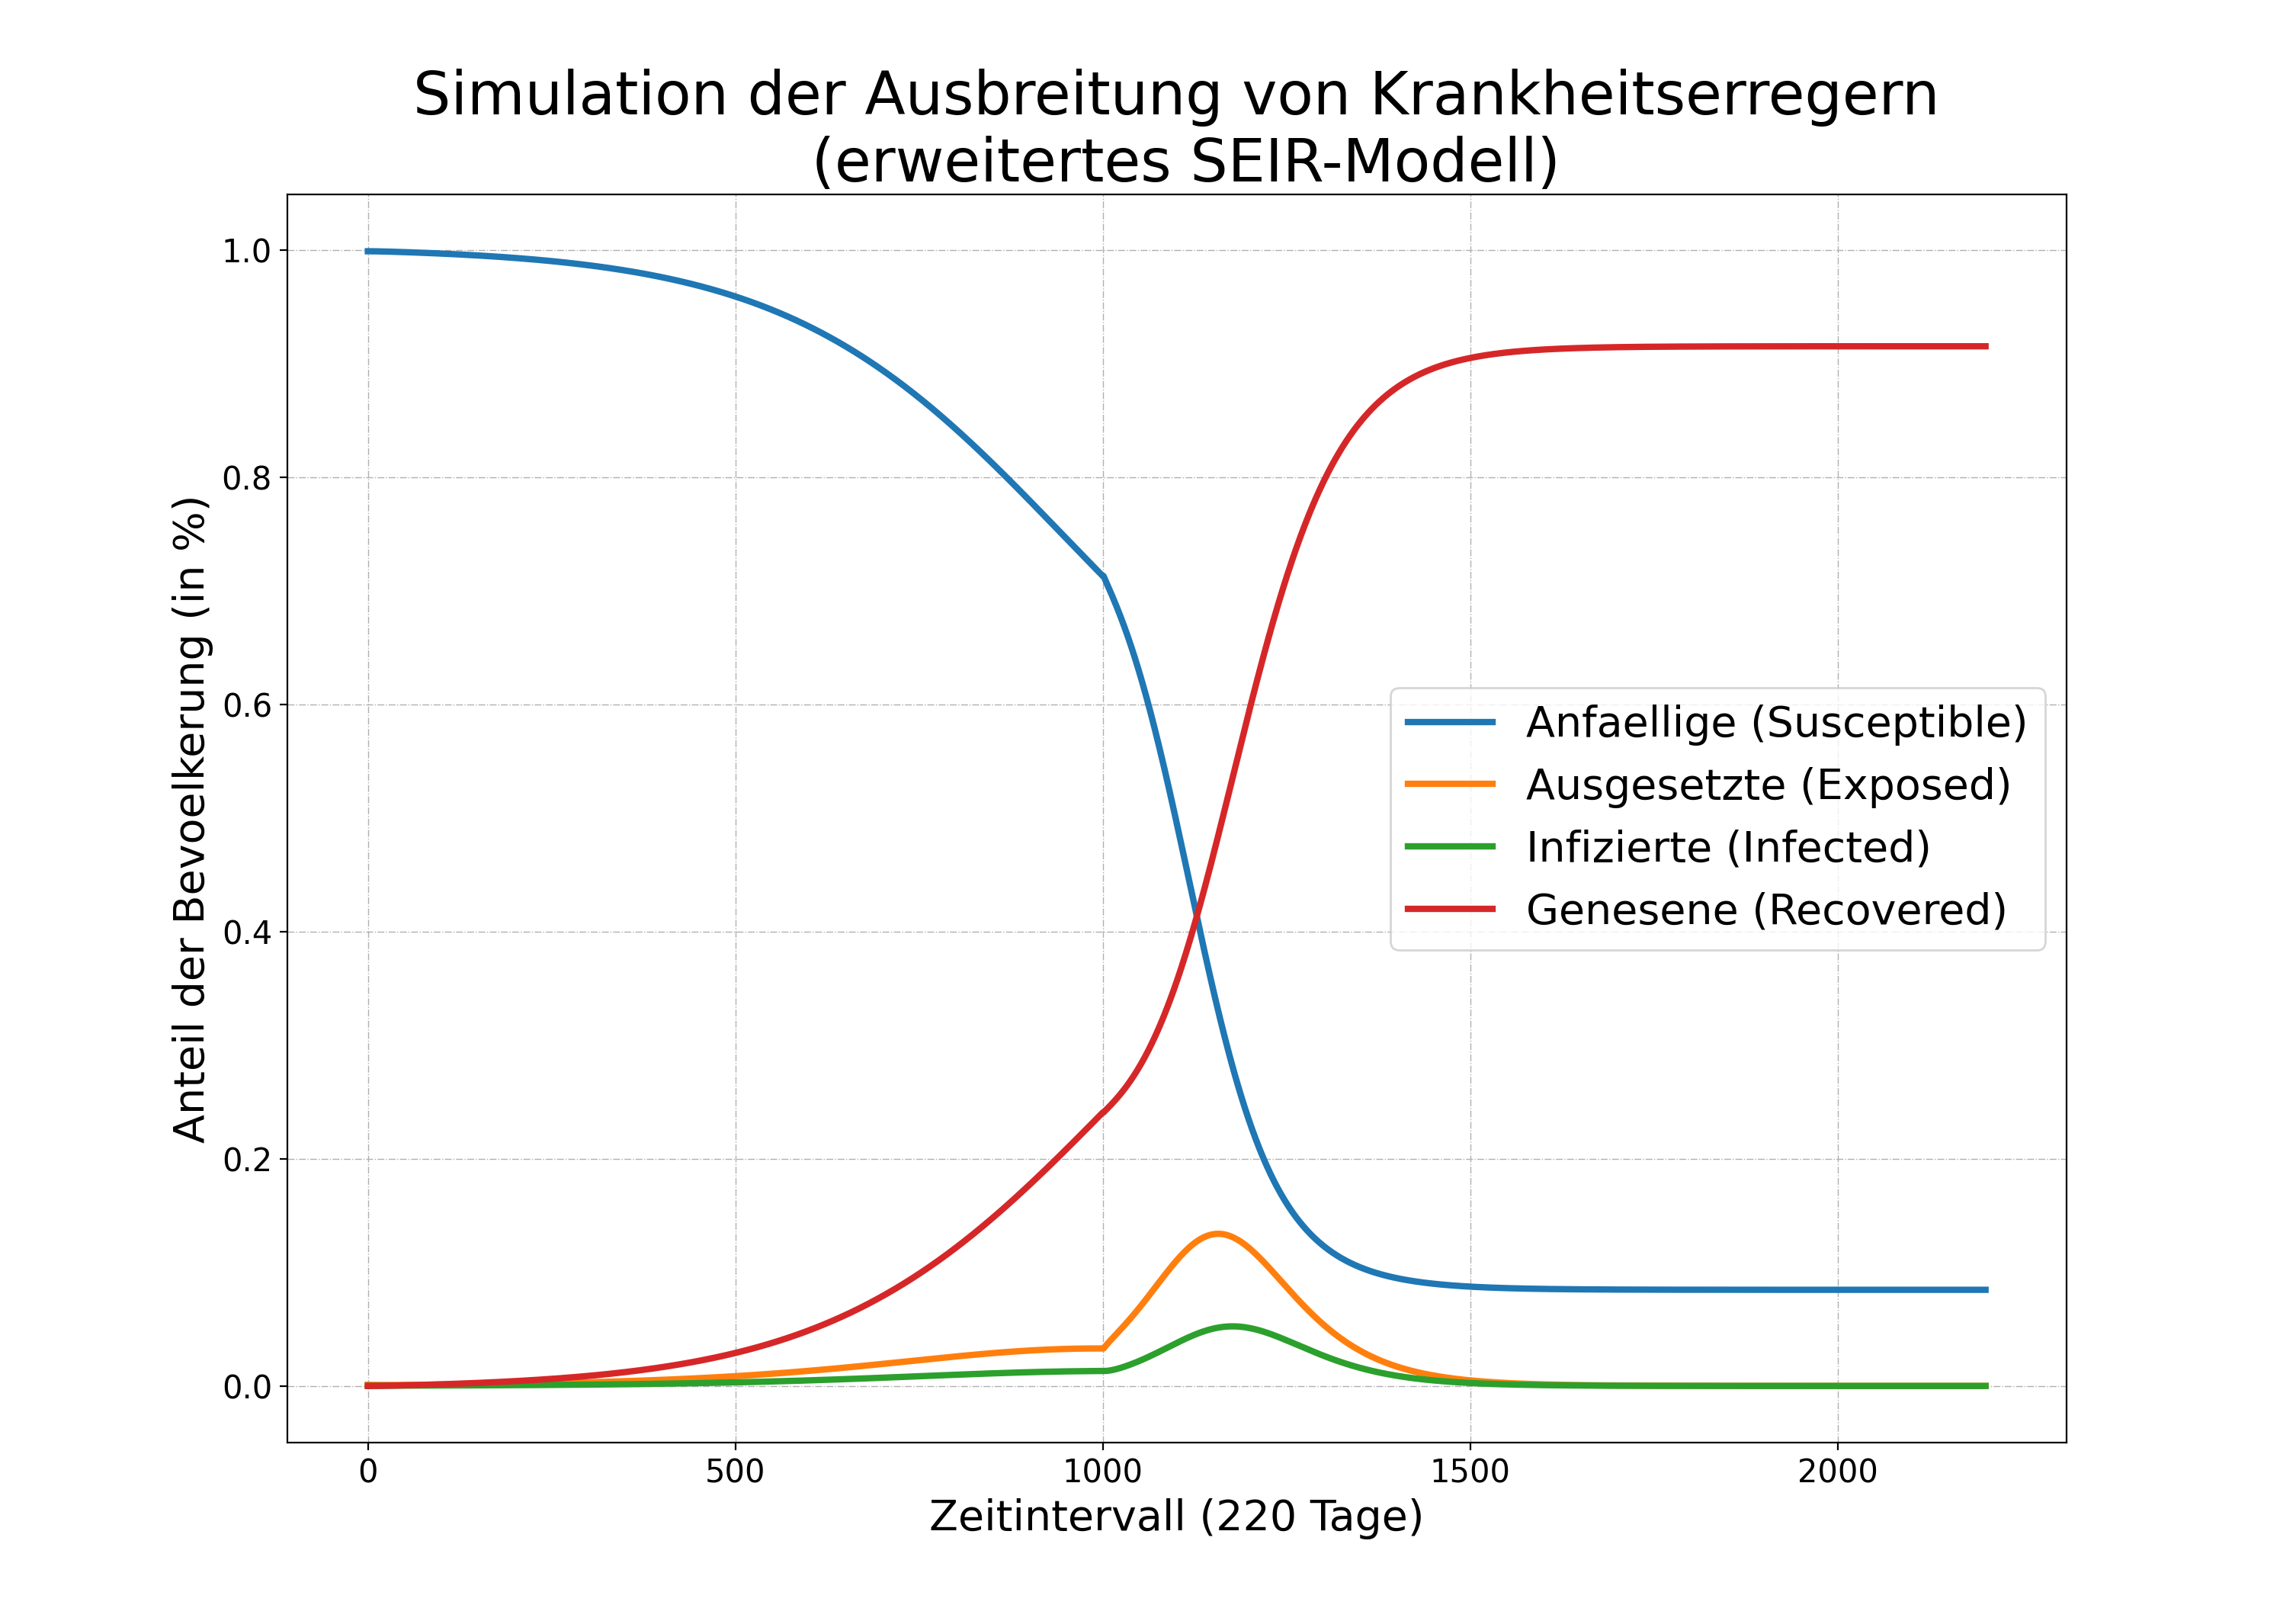
\includegraphics[scale=0.4]{Szenario_3}
\caption{Szenario 3 - Aufhebung eines Lockdown}
\label{fig:szenario_3}
\end{figure}

\begin{figure}[H]
\centering
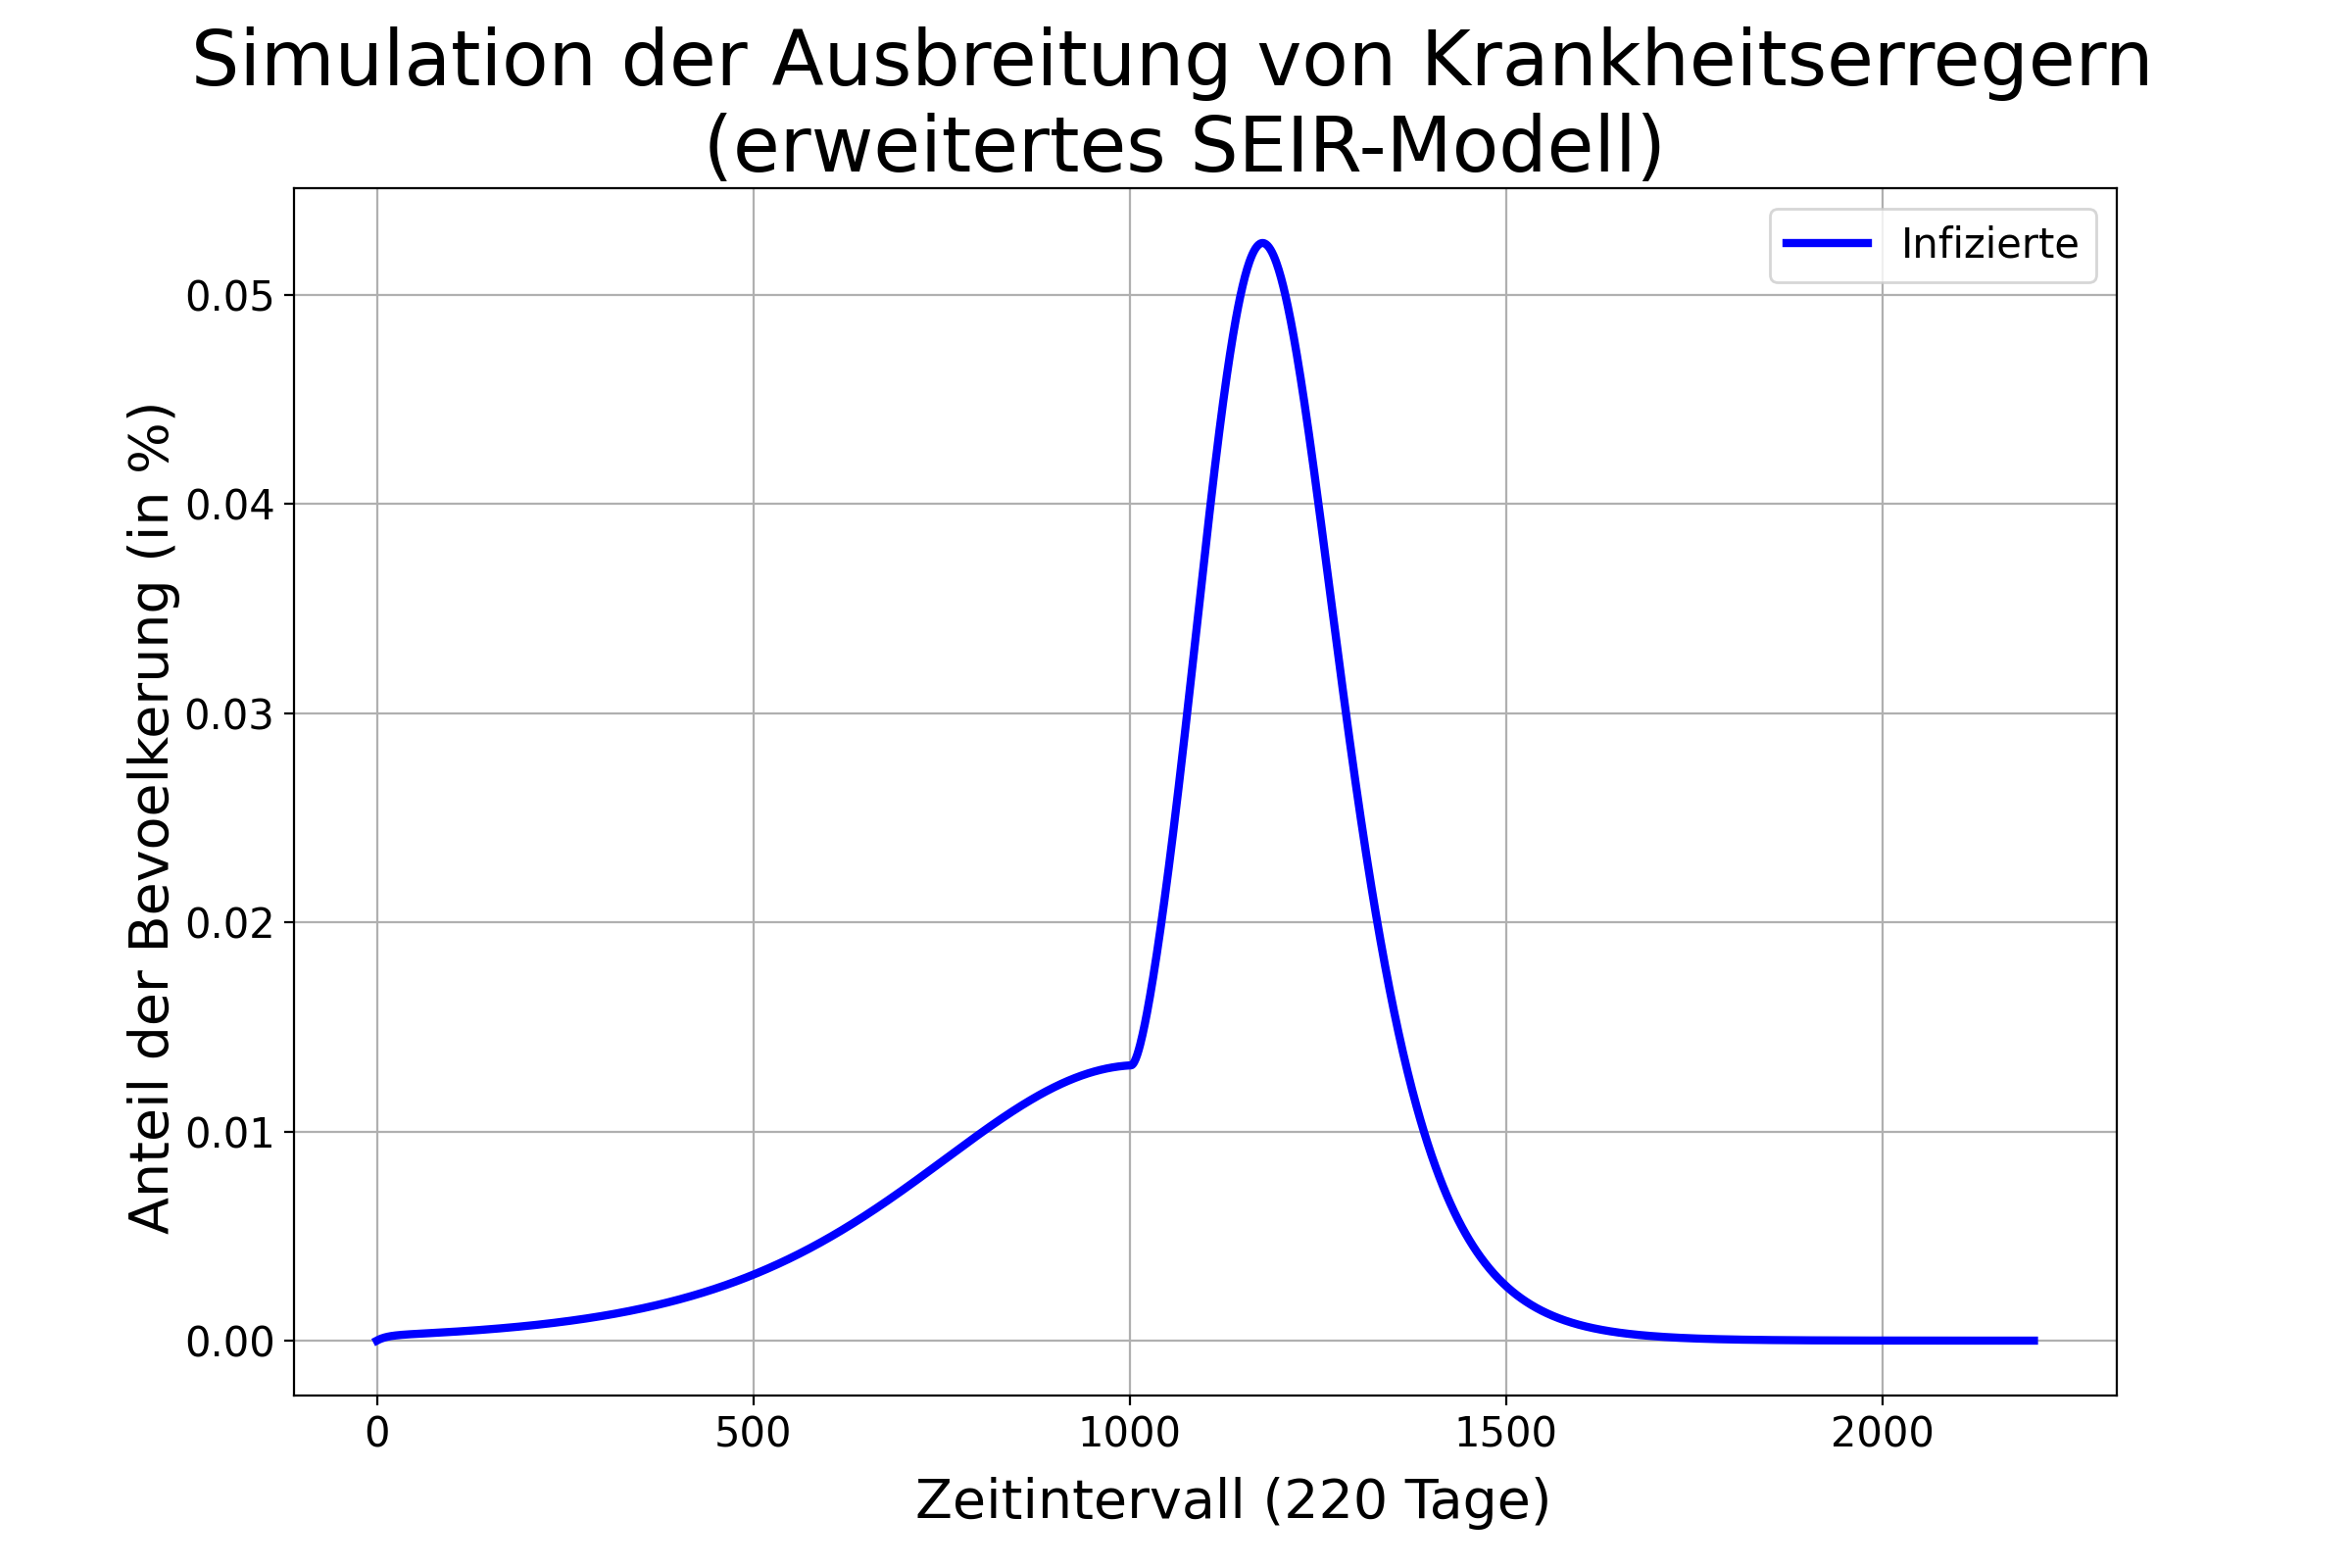
\includegraphics[scale=0.4]{Szenario_3_Infizierte}
\caption{Szenario 3 - Aufhebung eines Lockdown (Infizierte)}
\label{fig:szenario_3_Infizierte}
\end{figure}

\paragraph{Szenario 3.1 - „Lockdown aufgrund hoher Infektionszahlen“}
Im zweiten Fall des Szenarios (Listing \ref{lst:Szenario3.1} wird ein Lockdown aufgrund hoher Infektionszahlen aktiv. Das Vorgehen ist analog Listing \ref{lst:Szenario3} mit dem Unterschied, dass zuerst der niedrige Social Distancing-Faktor genutzt wird. Aus Szenario 1 ist bereits bekannt, dass die Anzahl der Infizierten, ohne Einschränkungen, stark ansteigt, deshalb wird für dieses Szenario der Lockdown bereits nach 15 Tagen aktiv\footnote{In Deutschland wurde im Jahre 2020 dieses Vorgehen als „harter Lockdown“ bezeichnet und durchgeführt.}. Teil eins der Simulation wird demnach auf 15 Tage begrenzt (Zeile 9). Der zweite Teil der Simulation wird wiederum mit den Werten aus Teil eins initialisiert (Zeile 10 - 11) und läuft für 120 Tage (Zeile 19). Vor der Anzeige der Gesamtsimulation (Zeile 21 -22) werden die Ergebnisse wieder verkettet (Zeile 20).

\begin{lstlisting}[language=Bash, caption=Szenario 3.1 - „Lockdown aufgrund hoher Infektionszahlen“, label=lst:Szenario3.1]
...
>>> modell.setze_parameter(parameter_=[0.2, 2.80, 0.5, 0.1], verbose=True)
Setzen der Parameter mit den folgenden Werten:
--------------------------------------------------
alpha (Inkubationszeit):    0.2
beta  (Uebertragunsrate):   1.75
gamma (Erholungszeit):      0.5
rho   (Social Distancing):  0.1
>>> result1 = modell.start(zeit_max=15, zeit_intervall=0.01)
>>> neu_init = modell.vals_
>>> modell2 = s.SEIR(initiale_werte=neu_init)
>>> modell2.setze_parameter(parameter_=[0.2, 1.75, 0.5, 0.6], verbose=True)
Setzen der Parameter mit den folgenden Werten:
--------------------------------------------------
alpha (Inkubationszeit):    0.2
beta  (Uebertragunsrate):   1.75
gamma (Erholungszeit):      0.5
rho   (Social Distancing):  0.6
>>> result2 = modell2.start(zeit_max=120, zeit_intervall=0.1, zuruecksetzen=False)
>>> result3 = np.vstack((result1,result2))
>>> modell2.zeichnen(result3, tage=135)
>>> modell2.zeichnen(result3[:,2], tage=135)
\end{lstlisting}

\begin{figure}[H]
\centering
\includegraphics[scale=0.4]{Szenario_3_Lockdown_Maßnahme}
\caption{Szenario 3 - Lockdown aufgrund hoher Infektionszahlen}
\label{fig:szenario_3_1}
\end{figure}

\paragraph{Einordnung Szenario 3}
Der erste Teil des Szenarios zeigt den zu erwartenden flachen Anstieg der Infektionen aufgrund des Social Distancing sowie den deutlichen Anstieg ab dem Ende des Lockdowns. Der bereits erhöhte Anfangswert im Vergleich zu Szenario 1 bewirkt einen steileren Anstieg der Infektionen. Dies wird besonders deutlich in Abbildung \ref{fig:szenario_3_Infizierte}, die nur die Kurze der Infizierten zeigt. Aus der Grafik lässt sich ableiten, dass ein zu frühes Aufheben des Lockdowns fatale Folgen, im Sinne der Infektionen, haben kann.

Im zweiten Teil des Szenarios steigen die Zahlen erwartungsgemäß rapide an. Erstaunlich ist, dass der Lockdown, trotz der hohen Anfangswerte unmittelbar Wirkung zeigt und in kürzester Zeit die Zahlen der Ausgesetzten und Infizierten rapide sinken. Wiederum zeigt sich, der bereits in Szenario 2 festgestellte Nachteil, dass die Zahö der Genesenen bei ca. 50\% stagnieren.

\subsection{Fazit der Simulationen}
Der Autor hat gezeigt, dass sich bereits mit wenigen Zeilen Code Simulationen mit erstaunlicher Bandbreite und erstem Erkenntnisgewinn erstellen lassen. So haben bereits diese einfachen Simulationen gezeigt, dass kleine Änderungen von wenigen Parametern große Auswirkungen haben. Ebenso ist erkennbar, das zu zu jeder Simulation eine Interpretation im Kontext erfolgen muss. Eine Vielzahl (an offensichtlichen) weiteren Fragestellungen drängen sich förmlich auf, würden aber den Rahmen dieser Arbeit bei weitem übersteigen. Für präzisere Simulationen sollte das Modell um weitere Parameter, z. B. für die Zahl der Geimpften oder für saisonale Unterschiede der Übertragungsrate, erweitert werden. Ebenfalls fehlen die Kurven zu Krankenhauseinweisungen und Todesfällen. Mit diesen Erweiterungen ist nach Meinung des Autors eine sinnvolle Berechnnug und Darstellung von Pandemien möglich.

\newpage
\section{Anhang (Codelisting)} \label{sec:Anhang}
\lstinputlisting[language=Python, caption=Python-Umsetzung des SEIR-Modells, label=PyUmsetzung]{SEIR_Simulation.py}
\newpage
\printbibliography
\end{document}